\section{Исследование управляемости}

Рассмотрим систему $\dot{x} = Ax + Bu$, где 
\begin{equation}
    \begin{array}{cc}
        A = \begin{bmatrix}
            5 & -2 & 8 \\
            4 & -3 & 4 \\
            -4 & 0 & -7
        \end{bmatrix}, &
        B = \begin{bmatrix}
            -7 \\
            -5 \\
            7
        \end{bmatrix}
    \end{array}
\end{equation}

\subsection{Управляемость системы}
\subsubsection{Матрица управляемости}
Найдем матрицу управляемости $U = [B, AB, A^2B]$: 
\begin{equation}
    U = \begin{bmatrix} 
        \begin{array}{c|c|c}
            \begin{bmatrix}
                -7 \\
                -5 \\
                7
            \end{bmatrix} & 
            \begin{bmatrix}
                5 & -2 & 8 \\
                4 & -3 & 4 \\
                -4 & 0 & -7
            \end{bmatrix} \times 
            \begin{bmatrix}
                -7 \\
                -5 \\
                7
            \end{bmatrix} &
            \begin{bmatrix}
                5 & -2 & 8 \\
                4 & -3 & 4 \\
                -4 & 0 & -7
            \end{bmatrix}^2 \times
            \begin{bmatrix}
                -7 \\
                -5 \\
                7
            \end{bmatrix}
        \end{array}   
    \end{bmatrix}
\end{equation}
\begin{equation}
    U = \begin{bmatrix}
        -7 & 31 & -43 \\
        -5 & 15 & -5 \\
        7 & -21 & 23 \\
    \end{bmatrix}
\end{equation}
Определим ранг матрицы управляемости:
\begin{equation}
    \text{rank}(U) = 3
\end{equation}
Так как ранг матрицы управляемости равен порядку системы, то система является полностью управляемой согласно критерию Калмана.

\subsubsection{Управляемость собственных значений}
Найдем спектр матрицы $A$:
\begin{equation}
    \sigma(A) = \{-3, -1-2j, -1+2j\}
\end{equation}

Для каждого собственного значения найдем матрицу Хаутуса $H_i = \begin{bmatrix} A - \lambda_i I & B \end{bmatrix}$ и определим ее ранг:
\begin{enumerate}
    \item $\lambda_1 = -3$: $H_1 = \begin{bmatrix}
        8 & -2 & 8 & -7\\
        4 & 0 & 4 & -5 \\
        -4 & 0 & -4 & 7
    \end{bmatrix}$, $\text{rank}(H_1) = 3$, собственное значение управляемо.
    \item $\lambda_2 = -1-2j$: $H_2 = \begin{bmatrix}
        6+2j & -2 & 8 & -7\\
        4 & -2+2j & 4 & -5 \\
        -4 & 0 & -6+2j & 7
    \end{bmatrix}$, $\text{rank}(H_2) = 3$, собственное значение управляемо.
    \item $\lambda_3 = -1+2j$: $H_3 = \begin{bmatrix}
        6-2j & -2 & 8 & -7\\
        4 & -2-2j & 4 & -5 \\
        -4 & 0 & -6-2j & 7
    \end{bmatrix}$, $\text{rank}(H_3) = 3$, собственное значение управляемо.
\end{enumerate}
Так как выше было показано, что система является полностью управляемой, то каждое собственное значение матрицы $A$ является управляемым. 

\subsubsection{Диагональная форма системы}
Найдем диагональную форму системы, заменив базис на базис из собственных векторов матрицы $A$:
\begin{equation}
    \dot{\hat{x}} = P^{-1}AP\hat{x} + P^{-1}Bu
\end{equation}
Где $P$ -- матрица собственных векторов матрицы $A$. 
Найдем собственные векторы матрицы $A$:
\begin{equation}
    \begin{array}{ccc}
        v_1 = \begin{bmatrix} -1 \\ 0 \\ 1 \end{bmatrix} &
        v_2 = \begin{bmatrix} -3+j \\ -2 \\ 2 \end{bmatrix} &
        v_3 = \begin{bmatrix} -3-j \\ -2 \\ 2 \end{bmatrix} 
    \end{array}
\end{equation}
Тогда матрица $P$:
\begin{equation}
    P = \begin{bmatrix}
        -1 & -3+j & -3-j \\
        0 & -2 & -2 \\
        1 & 2 & 2
    \end{bmatrix}
\end{equation}
Система преобразуется к виду:
\begin{equation}
    \dot{\hat{x}} = \begin{bmatrix}
        -3 & 0 & 0 \\
        0 & -1-2j & 0 \\
        0 & 0 & -1+2j
    \end{bmatrix} \hat{x} + 
    \begin{bmatrix}
        2 \\
        \frac{5 - 5j}{4} \\ 
        \frac{5 + 5j}{4}
    \end{bmatrix} u
\end{equation}
Так как все элементы $P^{-1}B$ не равны нулю, то система является полностью управляемой, каждая мода системы управляема.

\subsection{Грамиан управляемости}
Найдем грамиан управляемости $P(t_1)$:
\begin{equation}
    P(t_1) = \int_{0}^{t_1} e^{At}BB^Te^{A^Tt}dt
\end{equation}
Вычислим грамиан управляемости для $t_1 = 3$ с помощью функции \texttt{gram}: 
\begin{equation}
    P(3) = \begin{bmatrix}
        18.12 & 10.97 & -11.64 \\ 
        10.97 & 7.48 & -8.48 \\ 
        -11.64 & -8.48 & 10.14 \\ 
    \end{bmatrix}
\end{equation}
Найдем собственные числа Грамиана управляемости: 
\begin{equation}
    \sigma(P(3)) = \{ 0.05, 1.94, 33.74 \}
\end{equation}
Все собственные числа Грамиана управляемости положительны, что говорит о том, что система является управляемой.


\subsection{Управление системой}
Найдем управление $u(t)$, которое будет переводить систему из состояния $x(0) = 0$ в состояние $x_1 = x(t_1) = \begin{bmatrix} -2 & -3 & 3 \end{bmatrix}^T$. 
\begin{equation}
    u(t) = B^Te^{A^T(t_1 - t)}P(t_1)^{-1}x_1
\end{equation}
Реализуем данное управление в MATLAB и проведем моделирование системы. 
\begin{figure}
    \centering
    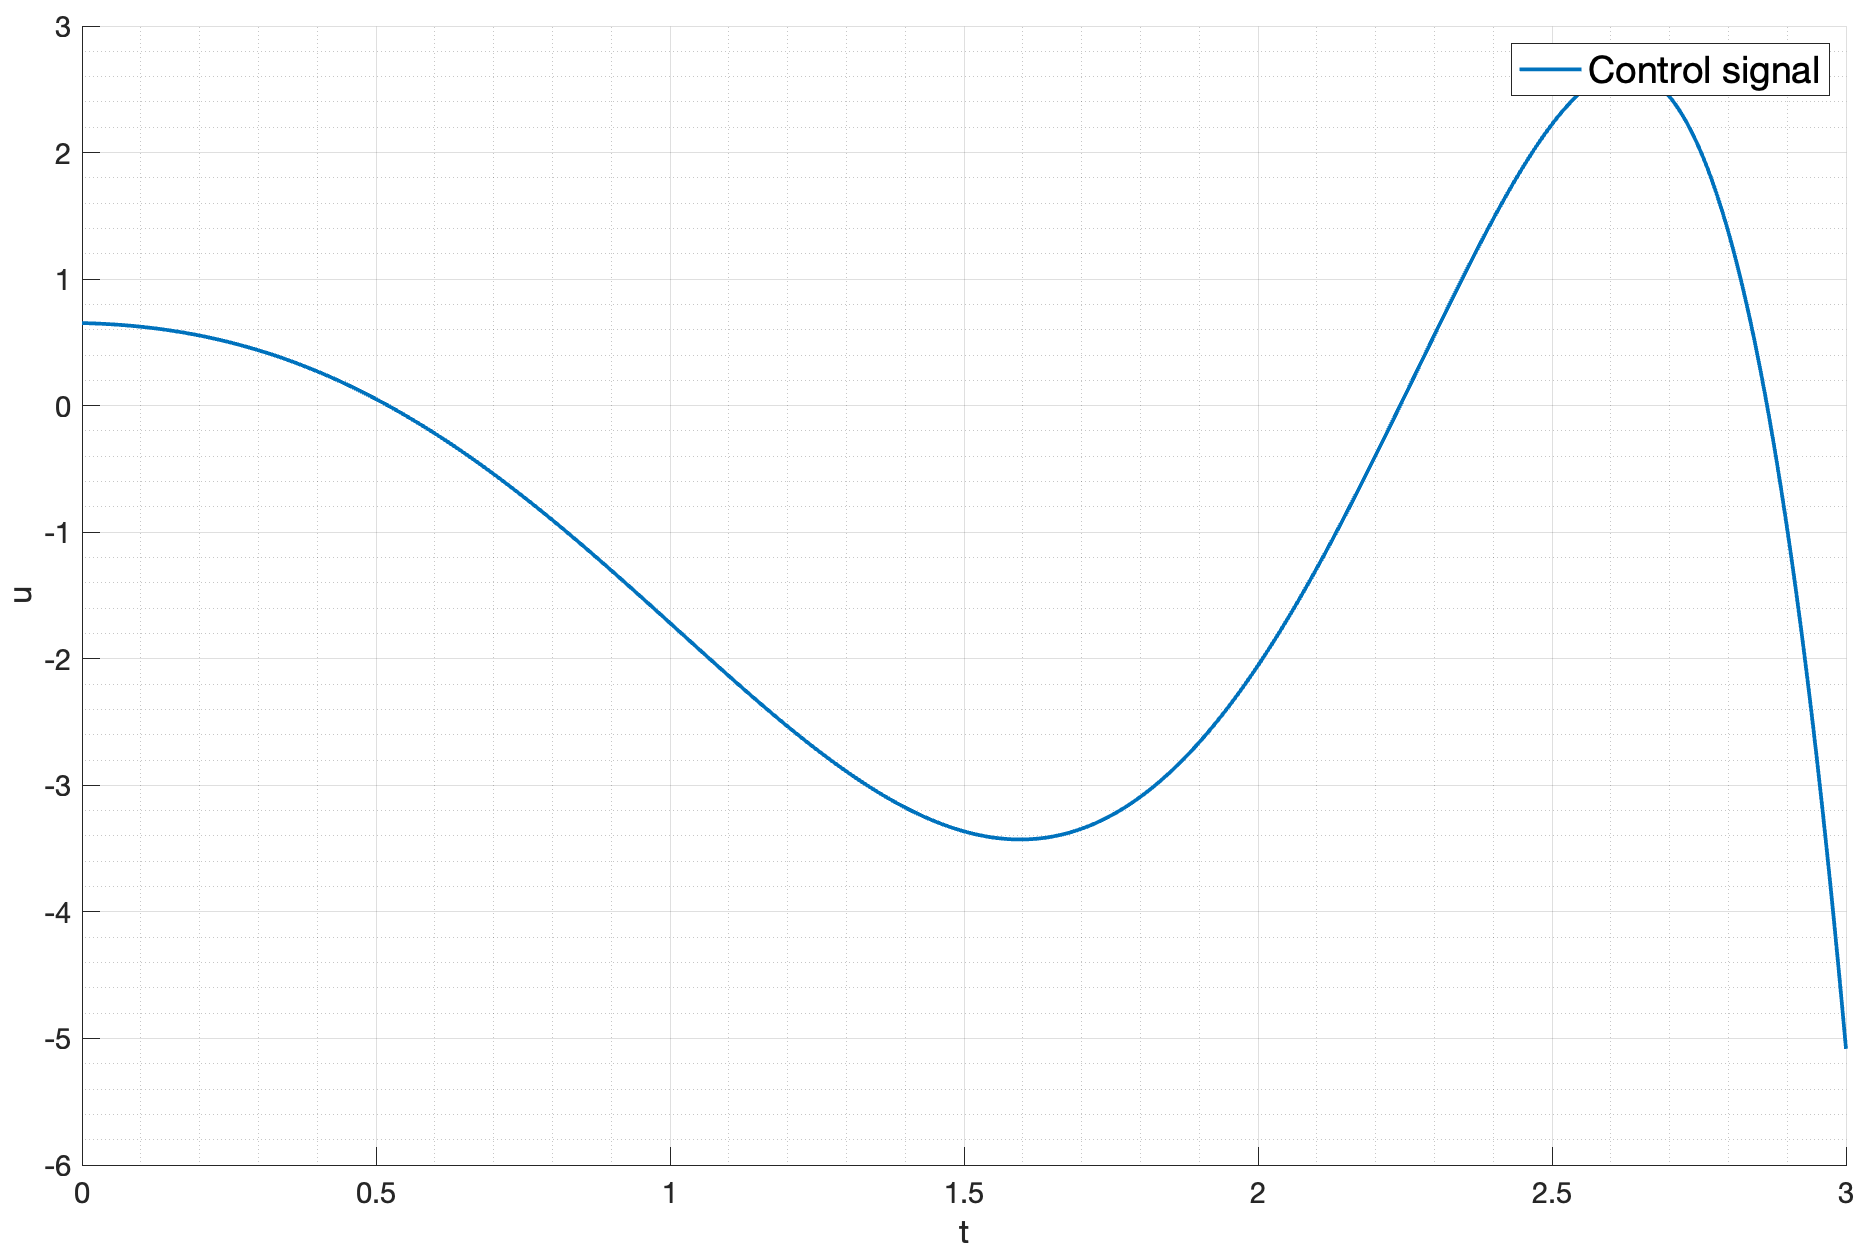
\includegraphics[width=\textwidth]{media/plots/task1_control_signal.png}
    \caption{Управление системой}
    \label{fig:task1_control_signal}
\end{figure}
На рисунке \ref{fig:task1_control_signal} изображено управление системой.
\begin{figure}
    \centering
    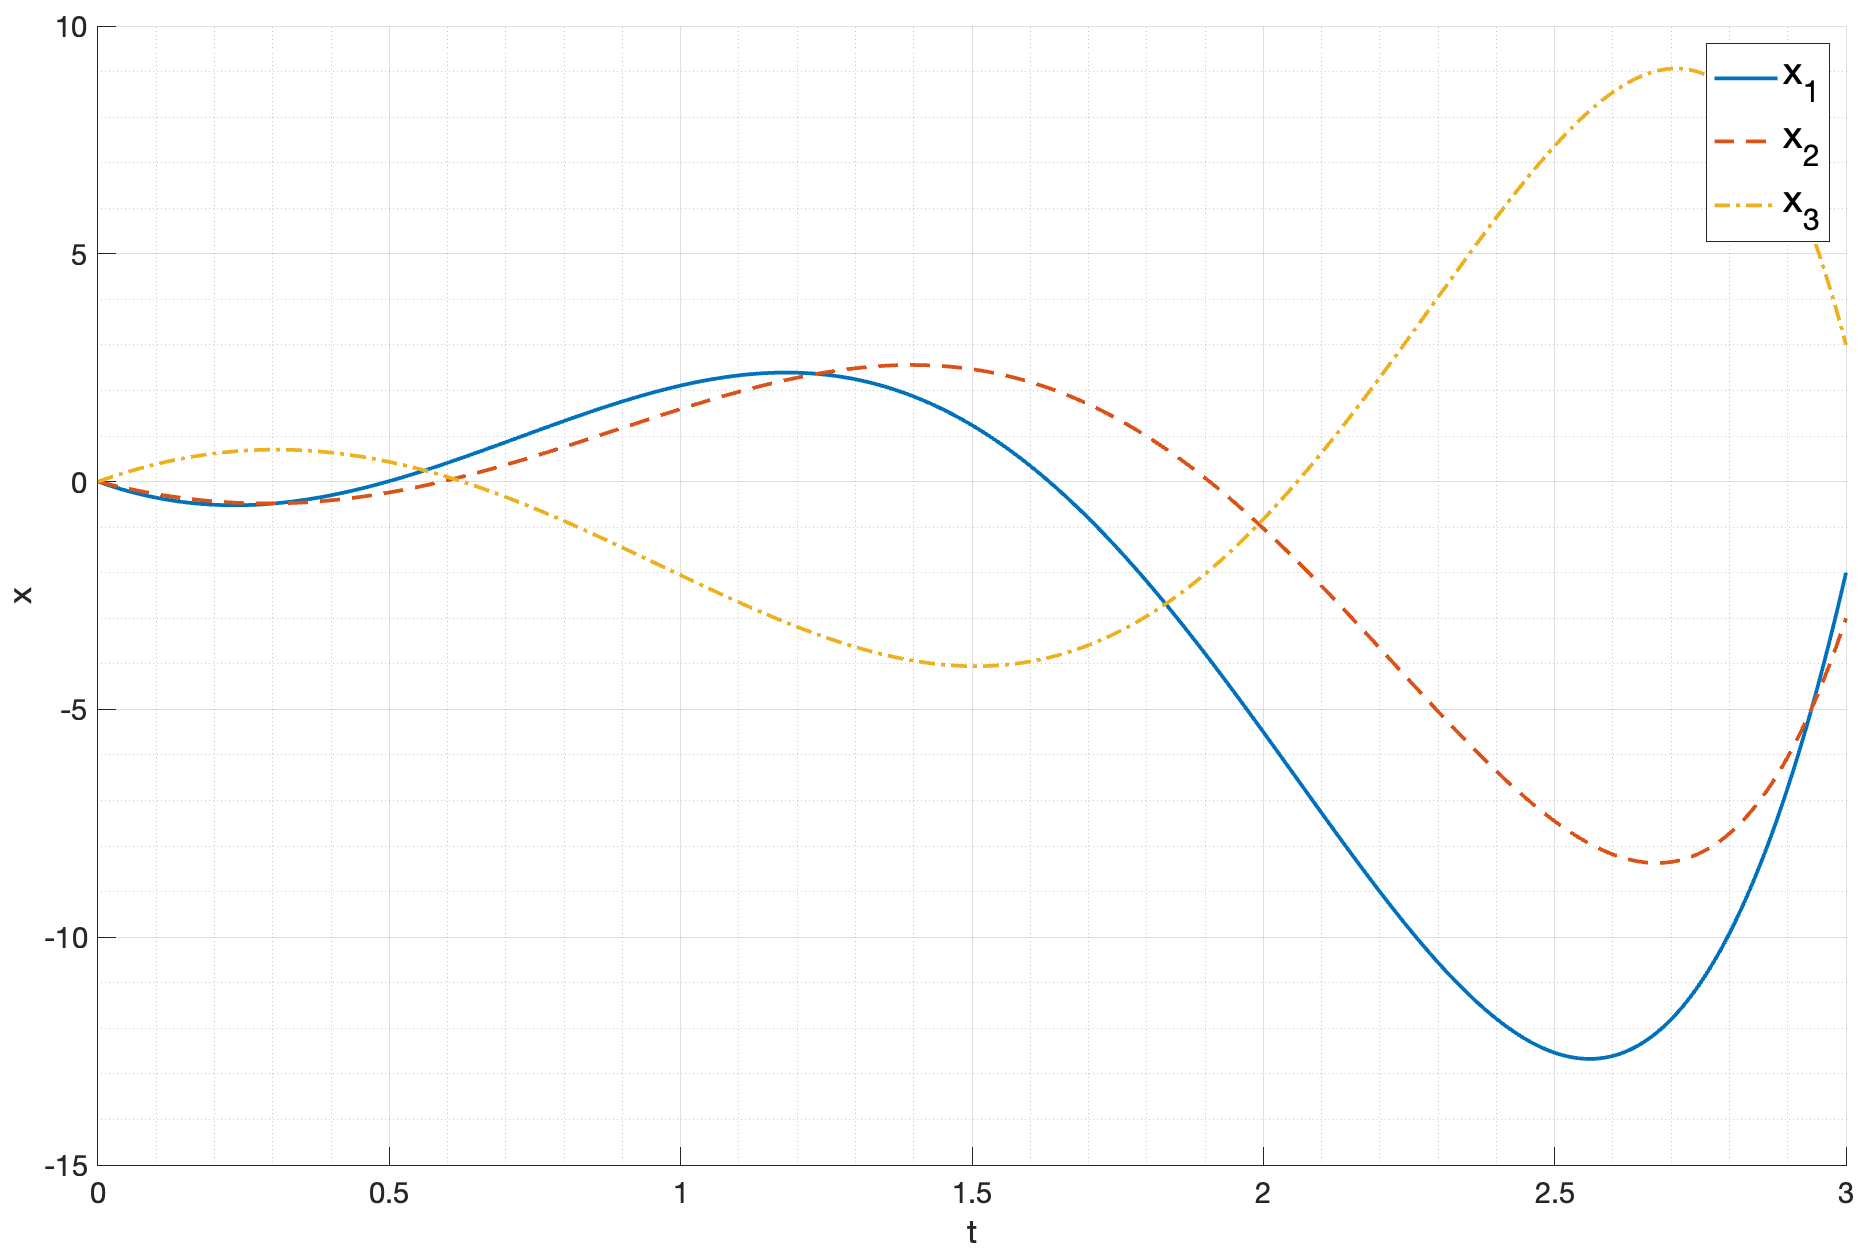
\includegraphics[width=\textwidth]{media/plots/task1_states.png}
    \caption{Состояние системы}
    \label{fig:task1_state}
\end{figure}
На рисунке \ref{fig:task1_state} изображено состояние системы.

Видно, что система управляемая в соответствии с заданным управлением и переходит в заданное состояние. 
\FloatBarrier
\subsection{Вывод}
При исследовании системы, рассматриваемой в этом заднии, удалось показать, что она является 
полностью управляемой. Это было продемонстрировано с помощью критерия Калмана, через 
управляемость собственных значений и диагональную форму системы. Также был найден грамиан 
управляемости и проверены его собственные числа. Проведено моделирование системы с управлением, 
которое переводит систему в заданное состояние. Результаты моделирования показали, что система
управляема и управление работает корректно. 
\FloatBarrier
\section{Управляемое подпространство}

Рассмотрим систему $\dot{x} = Ax + Bu$, где 
\begin{equation}
    \begin{array}{cc}
        A = \begin{bmatrix}
            5 & -2 & 8 \\
            4 & -3 & 4 \\
            -4 & 0 & -7
        \end{bmatrix}, &
        B = \begin{bmatrix}
            -1 \\
            -3 \\
            3
        \end{bmatrix}
    \end{array}
\end{equation}

\subsection{Управляемость системы}
\subsubsection{Матрица управляемости}
Найдем матрицу управляемости $U = [B, AB, A^2B]$:
\begin{equation}
    U = \begin{bmatrix} 
        \begin{array}{c|c|c}
            \begin{bmatrix}
                -1 \\
                -3 \\
                3
            \end{bmatrix} & 
            \begin{bmatrix}
                5 & -2 & 8 \\
                4 & -3 & 4 \\
                -4 & 0 & -7
            \end{bmatrix} \times 
            \begin{bmatrix}
                -1 \\
                -3 \\
                3
            \end{bmatrix} &
            \begin{bmatrix}
                5 & -2 & 8 \\
                4 & -3 & 4 \\
                -4 & 0 & -7
            \end{bmatrix}^2 \times
            \begin{bmatrix}
                -1 \\
                -3 \\
                3
            \end{bmatrix}
        \end{array}   
    \end{bmatrix}
\end{equation}
\begin{equation}
    U = \begin{bmatrix}
    -1 & 25 & -45 \\ 
    -3 & 17 & -19 \\ 
    3 & -17 & 19 \\ 
    \end{bmatrix}
\end{equation}
Определим ранг матрицы управляемости:
\begin{equation}
    \text{rank}(U) = 2
\end{equation}
Так как ранг матрицы управляемости меньше размерности матрицы $A$, система не является полностью управляемой. 

\subsubsection{Управляемость собственных значений}
Определим управляемость собственных значений матрицы $A$. Для каждого собственного значения найдем матрицу Хаутуса $H_i = \begin{bmatrix} A - \lambda_i I & B \end{bmatrix}$ и определим ее ранг:
\begin{enumerate}
    \item $\lambda_1 = -3$: $H_1 = \begin{bmatrix}
        8 & -2 & 8 & -1\\
        4 & 0 & 4 & -3 \\
        -4 & 0 & -4 & 3
    \end{bmatrix}$, $\text{rank}(H_1) = 2$, собственное значение не управляемо.
    \item $\lambda_2 = -1-2j$: $H_2 = \begin{bmatrix}
        6+2j & -2 & 8 & -1\\
        4 & -2+2j & 4 & -3 \\
        -4 & 0 & -6+2j & 3
    \end{bmatrix}$, $\text{rank}(H_2) = 3$, собственное значение управляемо.
    \item $\lambda_3 = -1+2j$: $H_3 = \begin{bmatrix}
        6-2j & -2 & 8 & -1\\
        4 & -2-2j & 4 & -3 \\
        -4 & 0 & -6-2j & 3
    \end{bmatrix}$, $\text{rank}(H_3) = 3$, собственное значение управляемо.
\end{enumerate}

\subsubsection{Диагональная форма системы}
\begin{equation}
    \dot{\hat{x}} = \begin{bmatrix}
        -3 & 0 & 0 \\
        0 & -1-2j & 0 \\
        0 & 0 & -1+2j
    \end{bmatrix} \hat{x} + 
    \begin{bmatrix}
        0 \\
        \frac{3 - 7j}{4} \\ 
        \frac{3 + 7j}{4}
    \end{bmatrix} u
\end{equation}
Первое число в векторе $P^{-1}B$ равно нулю, значит, что первое состояние системы не является управляемым. 
Результаты совпали с результатами, полученными при анализе управляемости собственных значений через матрицу Хаутуса.

\subsection{Грамиан управляемости}
Найдем грамиан управляемости $P(t_1)$:
\begin{equation}
    P(t_1) = \int_{0}^{t_1} e^{At}BB^Te^{A^Tt}dt
\end{equation}
Вычислим грамиан управляемости для $t_1 = 3$ с помощью функции \texttt{gram}: 
\begin{equation}
    P(3) = \begin{bmatrix}
        26.65 & 13.37 & -13.37 \\ 
        13.37 & 8.28 & -8.28 \\ 
        -13.37 & -8.28 & 8.28 \\ 
    \end{bmatrix}
\end{equation}
Найдем собственные числа Грамиана управляемости:
\begin{equation}
   \sigma(P(3)) = \{0, 2.03, 41.17 \}
\end{equation}
Первое собственное число равно нулю, что говорит о том, что Грамиан является вырожденным и система не является полностью
управляемой. Таким образом, для дальнейшего нахождения управления необходимо использовать псведообратную матрицу. 

\subsection{Управляемое подпространство}
Выясним, принадлежат ли точки $x_1'$ и $x_1''$ управляемому подпространству:
\begin{equation}
    \begin{array}{cc}
        x_1' = \begin{bmatrix}
            -2 \\
            -3 \\
            3
        \end{bmatrix}, &
        x_1'' = \begin{bmatrix}
            -3 \\
            -3 \\
            4
        \end{bmatrix}
    \end{array}
\end{equation}
Для этого можно записать расширенную матрицу управляемости $U'$ и найти ранг этой матрицы:
\begin{equation}
    U' = \begin{bmatrix}
        -1 & 25 & -45 & -2 \\
        -3 & 17 & -19 & -3 \\
        3 & -17 & 19 & 3
    \end{bmatrix}
\end{equation}
\begin{equation}
    \text{rank}(U') = 2
\end{equation}

\begin{equation}
   U'' = \begin{bmatrix}
        -1 & 25 & -45 & -3 \\
        -3 & 17 & -19 & -3 \\
        3 & -17 & 19 & 4
    \end{bmatrix}
\end{equation}
\begin{equation}
    \text{rank}(U'') = 3
\end{equation}
Таким образом, можно сделать вывод, что точка $x_1'$ принадлежит управляемому подпространству, а точка $x_1''$ не принадлежит. В дальнейшем будем обозначать $x_1'$ как $x_1$.

\subsection{Управление системой}
Найдем управление $u(t)$, которое будет переводить систему из состояния $x(0) = 0$ в состояние $x_1 = x(t_1) = \begin{bmatrix} -2 & -3 & 3 \end{bmatrix}^T$. 
\begin{equation}
    u(t) = B^Te^{A^T(t_1 - t)}P(t_1)^{-1}x_1
\end{equation}
Реализуем данное управление в MATLAB и проведем моделирование системы.  
\begin{figure}
    \centering
    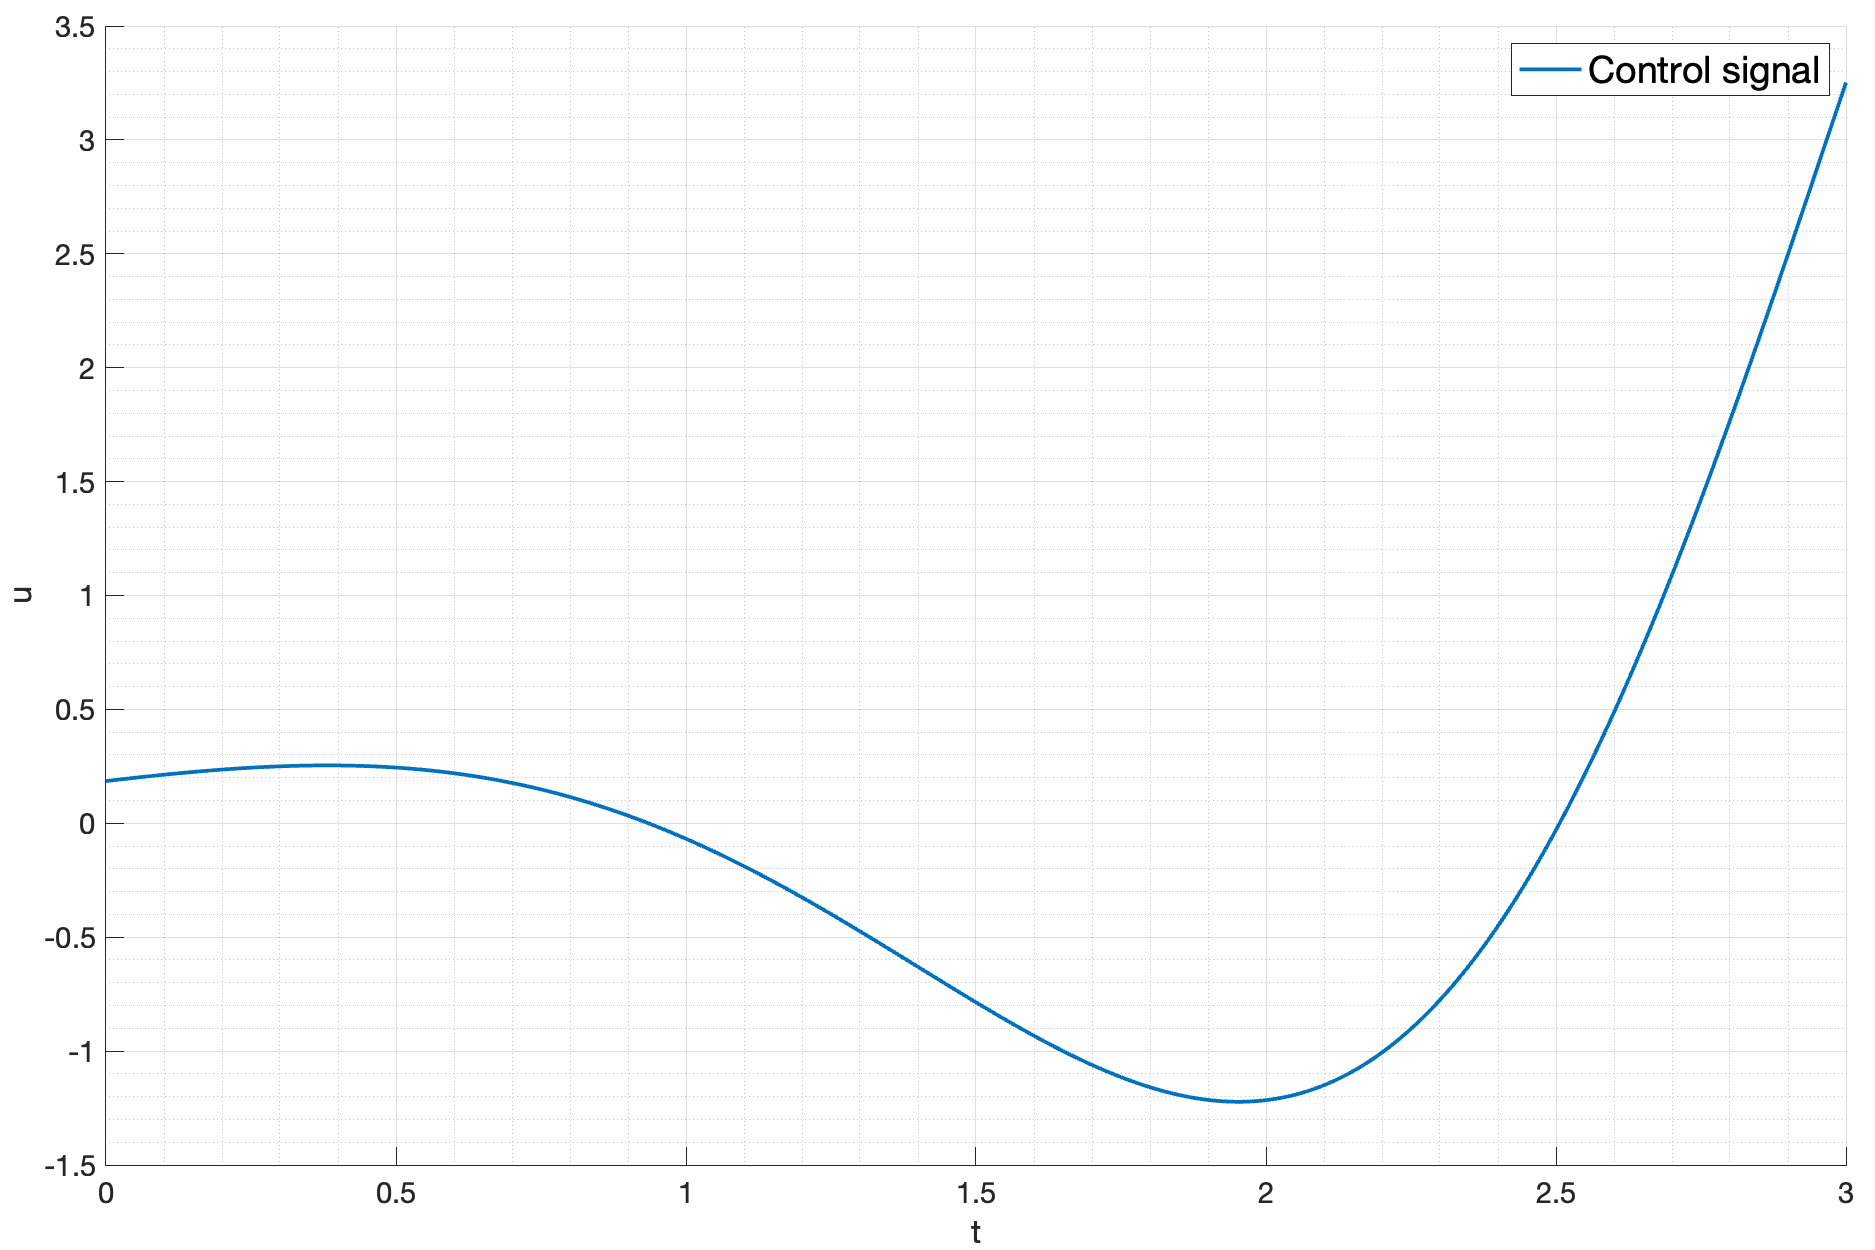
\includegraphics[width=\textwidth]{media/plots/task2_control_signal.png}
    \caption{Управление системой}
    \label{fig:task2_control_signal}
\end{figure}
На рисунке \ref{fig:task2_control_signal} изображено управление системой.
\begin{figure}
    \centering
    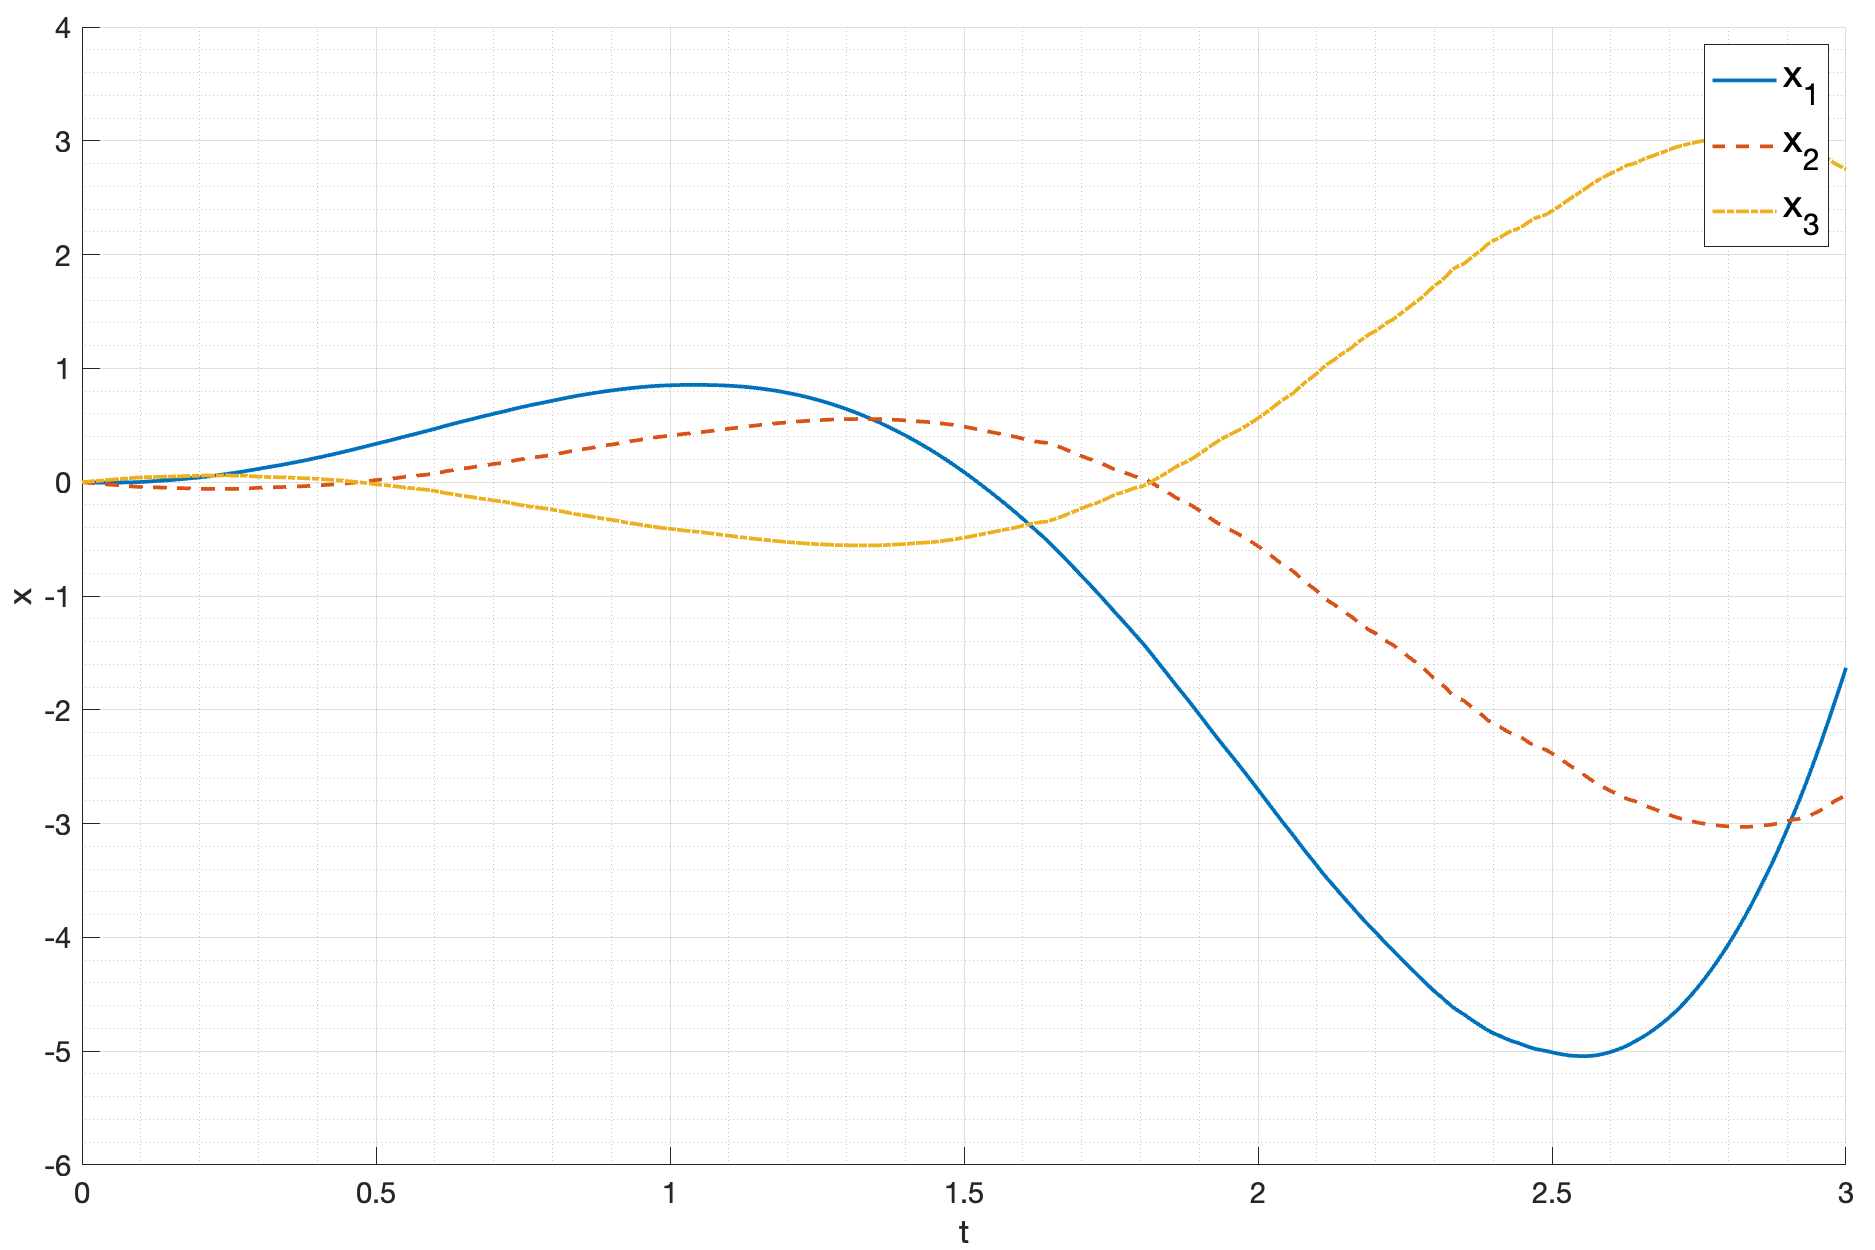
\includegraphics[width=\textwidth]{media/plots/task2_states.png}
    \caption{Состояние системы}
    \label{fig:task2_state}
\end{figure}
На рисунке \ref{fig:task2_state} изображено состояние системы.

Видно, что система управляемая в соответствии с заданным управлением и переходит в заданное состояние. 

\FloatBarrier
\subsection{Вывод}
При исследовании системы, рассматриваемой в этом задании, получилось доказать, что она 
не является полностью управляемой. Это было продемонстрировано с помощью критерия Калмана,
через управляемость собственных значений и диагональную форму системы. При этом оказалось, 
что собственное число $\lambda_1 = -3$ не является управляемым. Также был найден грамиан
управляемости и проверены его собственные числа. Одно из собственных чисел равно нулю, что
говорит о том, что система не является полностью управляемой. 

Были рассмотрены две точки $x_1'$ и $x_1''$ и проверена их принадлежность управляемому
подпространству. Точка $x_1'$ принадлежит управляемому подпространству, а точка $x_1''$ не принадлежит. 
Проведено моделирование системы с управлением, которое переводит систему в заданное состояние.
Результаты моделирования показали, что система управляема и управление работает корректно.
\FloatBarrier
\section{Регулятор с качественной экспоненциальной устойчивостью}
Рассмотрим систему: 
\begin{equation}
    \dot{x} = Ax + Bu
\end{equation}
где 
\begin{equation}
    \begin{array}{cc}
        A = \begin{bmatrix}
            8 & 1 & 11 \\ 
            4 & 0 & 4 \\
            -4 & -3 & -7
        \end{bmatrix}, &
        B = \begin{bmatrix}
            -1 \\ -3 \\ 3
        \end{bmatrix}
    \end{array}
\end{equation}


Для определения управляемости собственных чисел рассмотрим вещественную Жорданову форму системы: 
\begin{equation}
    \dot{\hat{x}} = P^{-1}AP\hat{x} + P^{-1}Bu
\end{equation}
Где $P$ -- матрица собственных векторов матрицы $A$, а $\hat{x} = P^{-1}x$.
\begin{equation}
    A_j = \begin{bmatrix}
        -3  & 0  & 0 \\ 
        0  & 2  & -2 \\ 
        0  & 2  & 2 \\ 
    \end{bmatrix}\quad
    P = \begin{bmatrix}
        -1  & -2.12  & 0.71 \\ 
        0  & -1.41  & 0 \\ 
        1  & 1.41  & 0 \\ 
    \end{bmatrix}\quad 
    B_j = \begin{bmatrix}
        0 \\ 
        2.12 \\ 
        4.95 \\ 
    \end{bmatrix}
\end{equation}

Таким образом, последнее собственное число $\lambda_3 = -3$ не является управляемым. Соответственно, система не является полностью управляемой. 
Но, так как данное собственное число располагается в левой полуплоскости, то есть является устойчивым, то система является стабилизируемой. 

\subsection{Синтез регулятора}
Зададимся значением $\beta = -4$ как средним значением поведения траектории системы 
и параметром $r = 2$, характеризующим разброс разброс поведения траектории 
относительно значения $\beta$.

С помощью матричного уравнения Риккати синтезируем регулятор $K$: 
\begin{eqnarray}
    (A - Bk - \beta I)^TP(A - Bk - \beta I) - r^2P = -Q, & K = (-R + B^T PB)^{-1}B^TP(A - \beta I)
\end{eqnarray}
для каждой из пар значений $Q$ и $R$:
\begin{enumerate}
    \item $Q = I, R = 1$
    \item $Q = I, R = 0$ 
    \item $Q = 0, R = 1$
    \item $Q = 0, R = 0$
\end{enumerate}

Полученные значения матрицы $K_i$:
\begin{equation}
    \begin{array}{cccc}
        K_1 = \begin{bmatrix}
            -3.10  & 0.98  & -3.10 \\ 
        \end{bmatrix} \\
        K_2 = \begin{bmatrix}
            -3.16  & 1.00  & -3.16 \\ 
        \end{bmatrix} \\
        K_3 = \begin{bmatrix}
            -3.29  & 1.14  & -3.29 \\ 
        \end{bmatrix} \\ 
        K_4 = \begin{bmatrix}
            -4.29  & 1.00  & -4.29 \\
        \end{bmatrix}
    \end{array}
\end{equation}
Для каждой системы, замкнутой регулятором $K_i$, найдем собственные числа матрицы $A - BK_i$: 
\begin{equation}
    \begin{array}{cccc}
        \sigma_1 = \begin{bmatrix}
            -2.57 + 0.58j \\ 
            -2.57 - 0.58j \\ 
            -3.00 \\ 
        \end{bmatrix} & 
        \sigma_2 = \begin{bmatrix}
            -3.00 \\ 
            -2.32 \\ 
            -3.00 \\ 
        \end{bmatrix} &
        \sigma_3 = \begin{bmatrix}
            -2.62 + 1.96j \\ 
            -2.62 - 1.96j \\ 
            -3.00 \\ 
        \end{bmatrix} &
        \sigma_4 = \begin{bmatrix}
            -3.00 \\ 
            -3.00 \\ 
            -4.58 \\ 
        \end{bmatrix}
    \end{array}
\end{equation}

Построим окружность на комплексной плоскости с центром в точке $(\beta, 0)$ и радиусом $r$, 
на этой же плоскости разместим собственные числа системы, замкнутой по регулятору $K_i$. 
Полученные графики представлены на рисунке \ref{fig:task3_eigs1} -- \ref{fig:task3_eigs4}.

\begin{figure}[ht!]
    \centering
    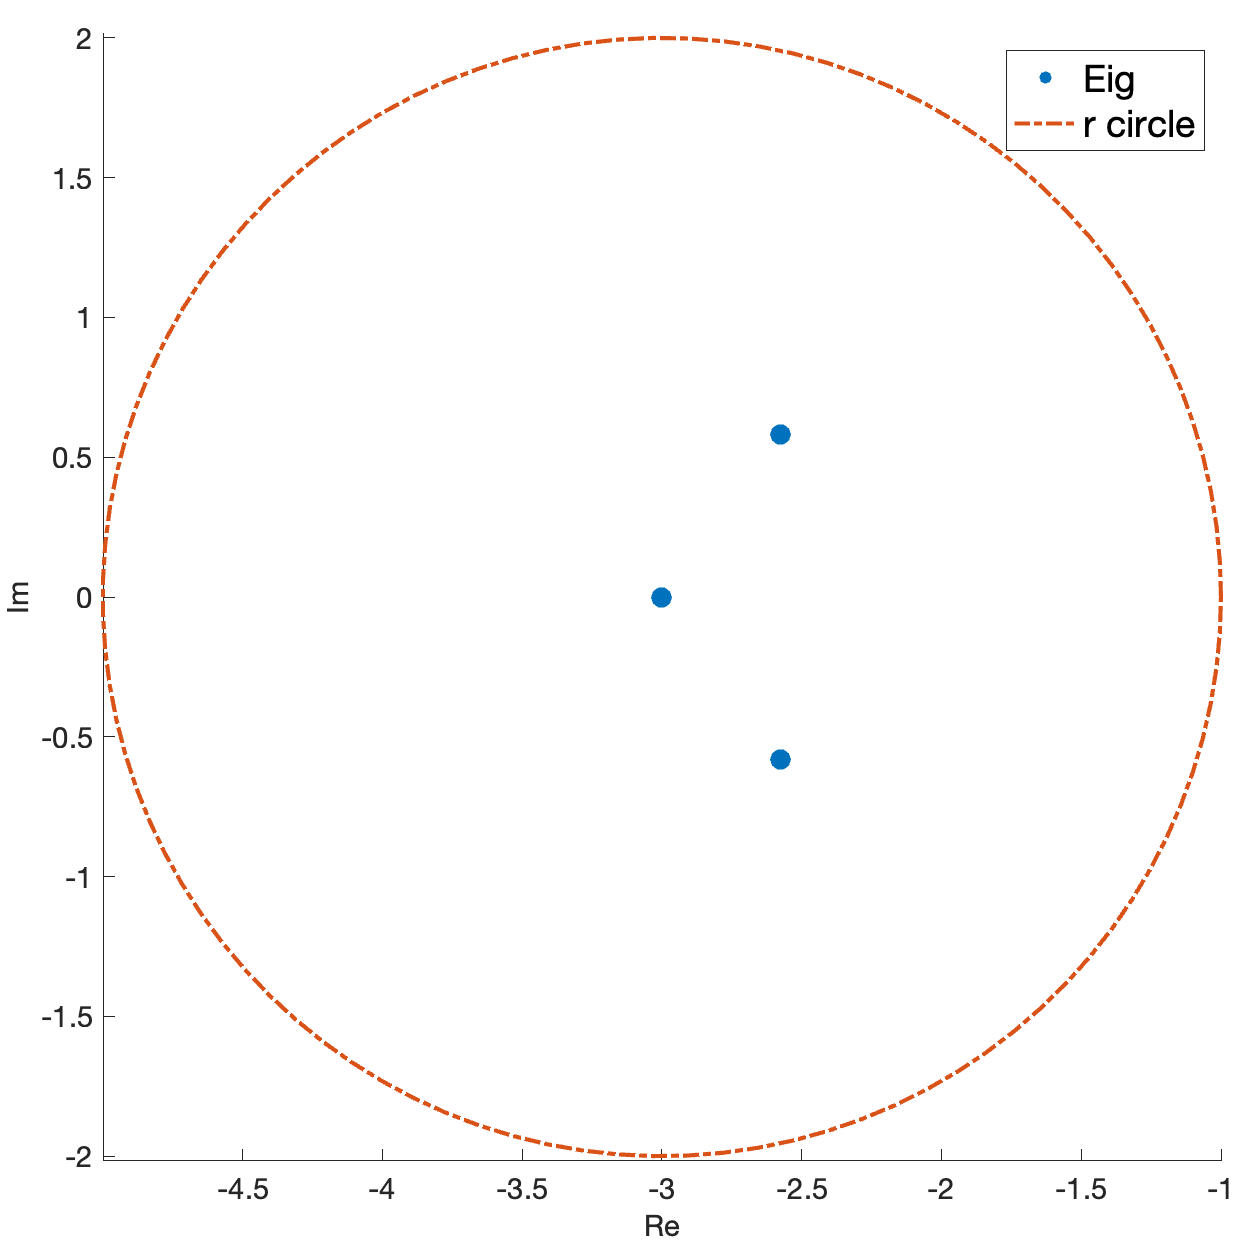
\includegraphics[width=0.7\textwidth]{media/plots/task3_eigs_1.png}
    \caption{Собственные числа системы, замкнутой по регулятору $K_1$}
    \label{fig:task3_eigs1}
\end{figure}
\begin{figure}[ht!]
    \centering
    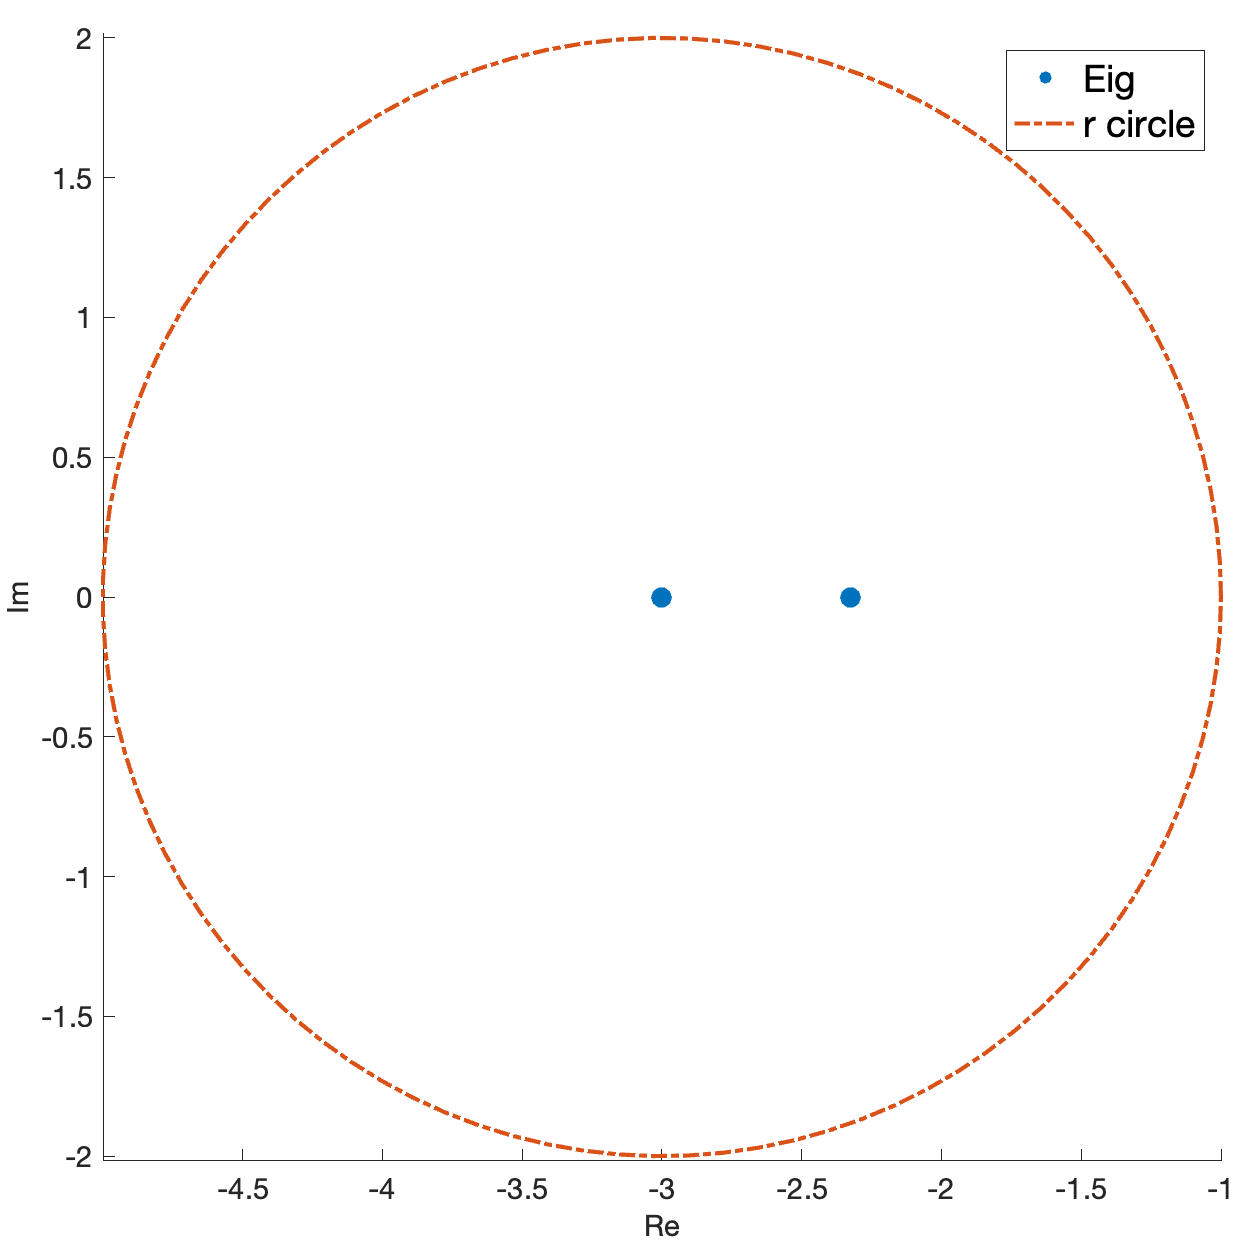
\includegraphics[width=0.7\textwidth]{media/plots/task3_eigs_2.png}
    \caption{Собственные числа системы, замкнутой по регулятору $K_2$}
    \label{fig:task3_eigs2}
\end{figure}
\begin{figure}[ht!]
    \centering
    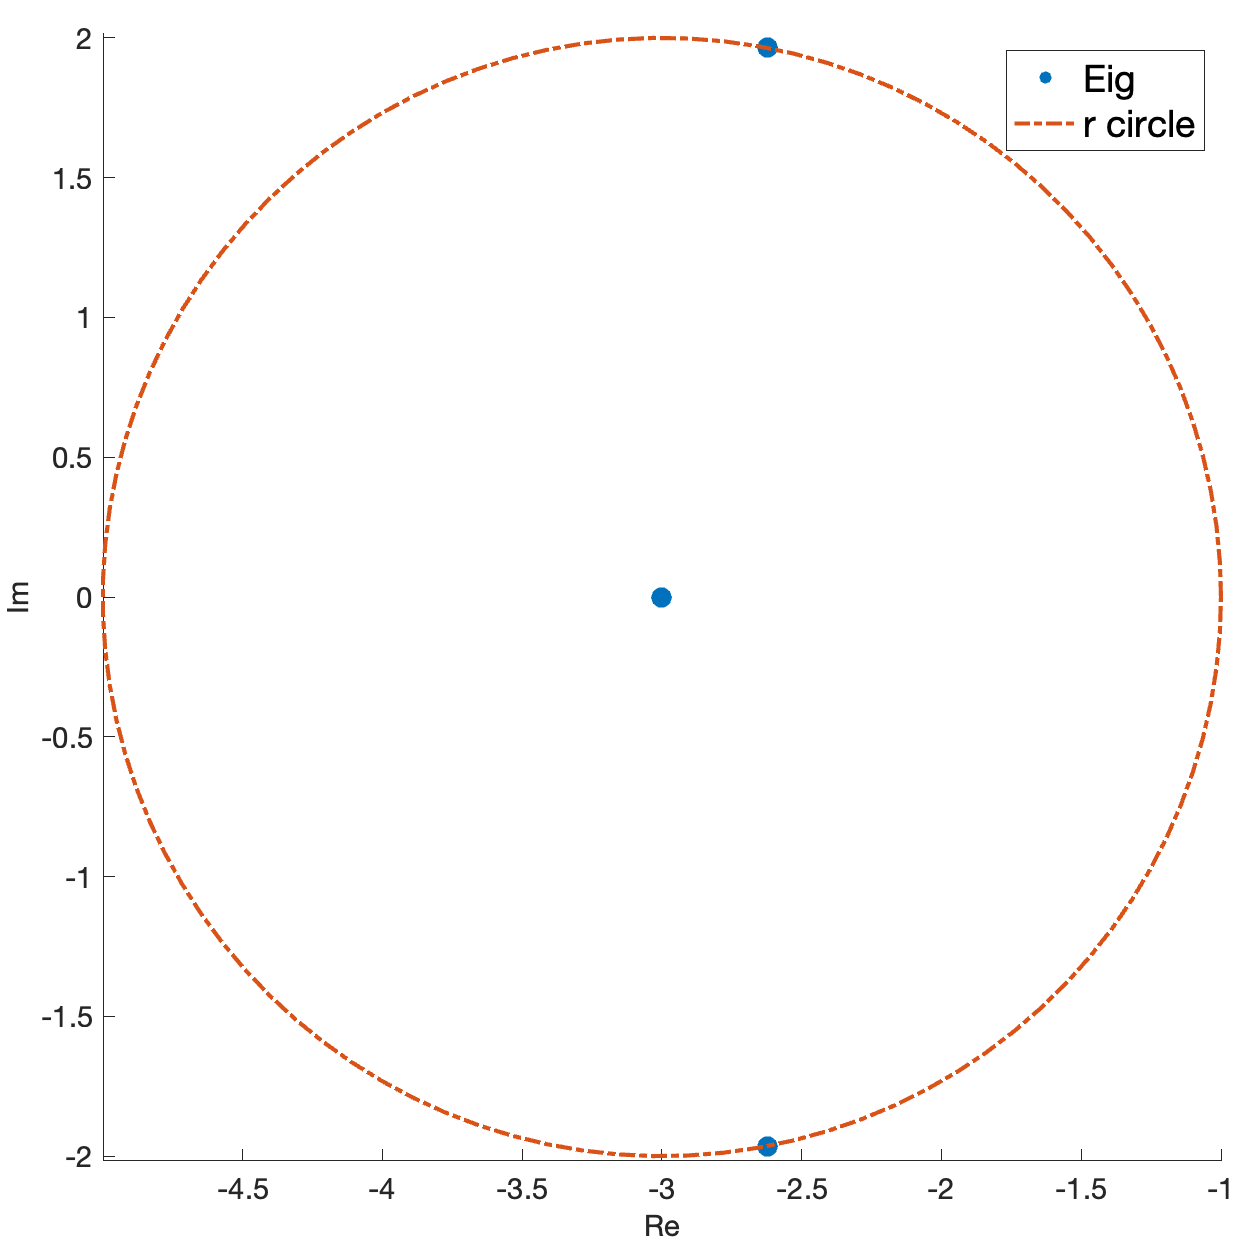
\includegraphics[width=0.7\textwidth]{media/plots/task3_eigs_3.png}
    \caption{Собственные числа системы, замкнутой по регулятору $K_3$}
    \label{fig:task3_eigs3}
\end{figure}
\begin{figure}[ht!]
    \centering
    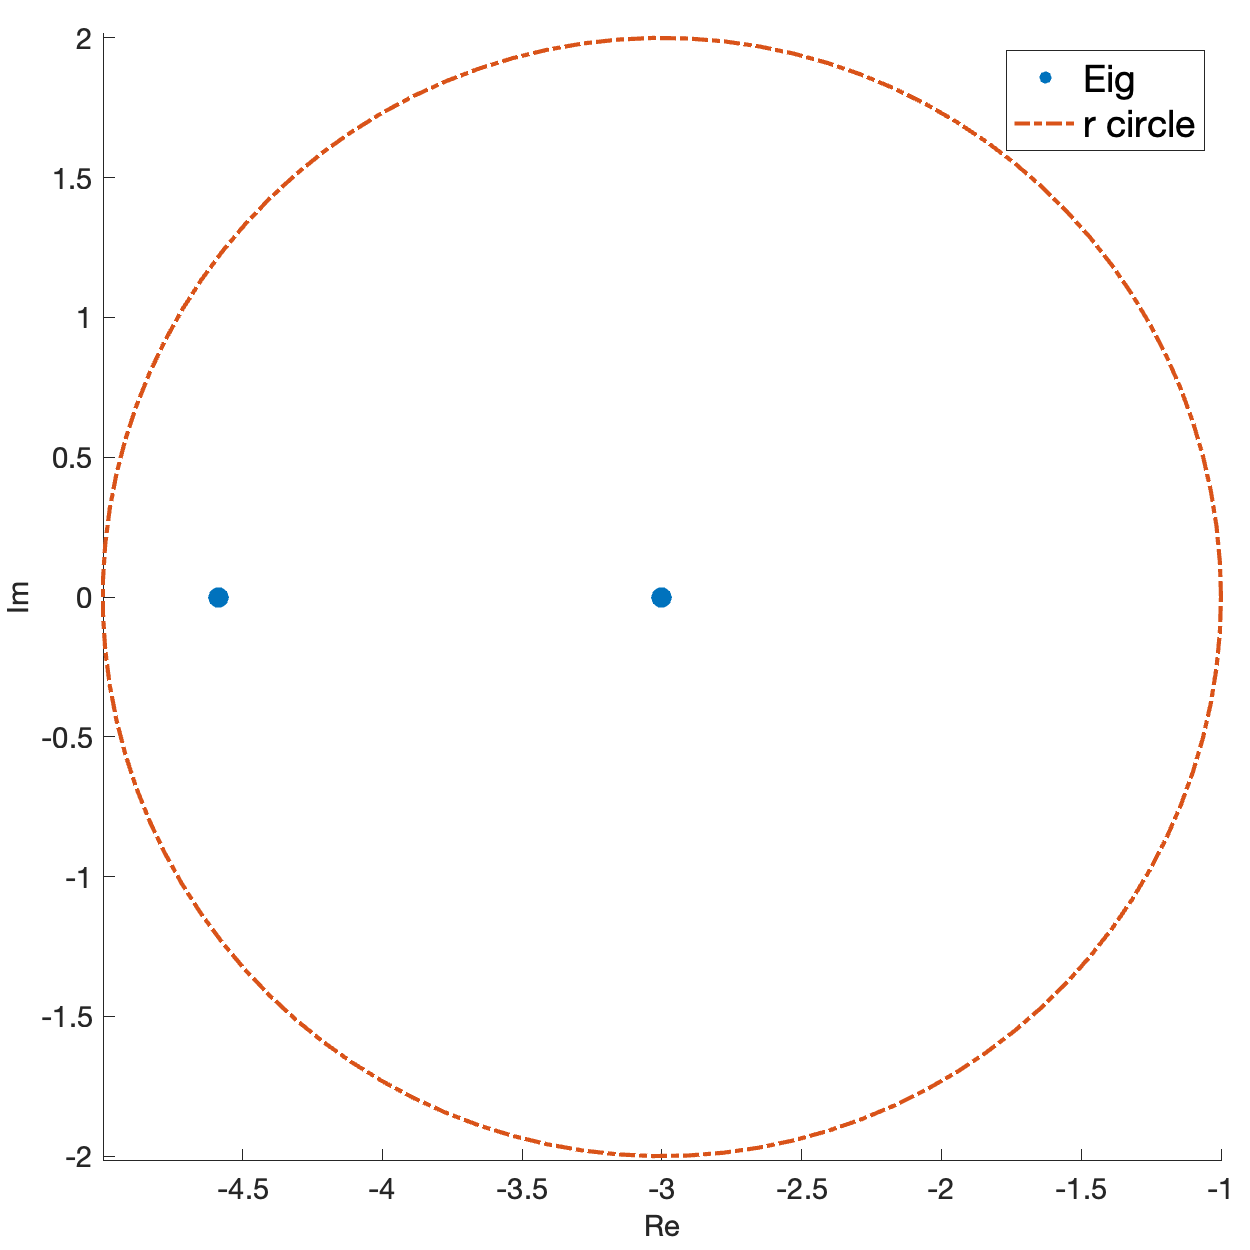
\includegraphics[width=0.7\textwidth]{media/plots/task3_eigs_4.png}
    \caption{Собственные числа системы, замкнутой по регулятору $K_4$}
    \label{fig:task3_eigs4}
\end{figure}

Видно, что во всех случаях полученные собственные числа замкнутой регулятором 
системы располагаются внутри окружности, что подтверждает, что полученные регуляторы 
обеспечивают качественную экспоненциальную устойчивость системы. 

\subsection{Моделирование}
Проведем моделирование систем, замкнутых по регуляторам $K_i$. 

Для системы с регулятором $K_1$ результаты моделирования представлены на рисунке \ref{fig:task3_x} 
(состояние системы) и \ref{fig:task3_1_u} (управляющее воздействие).

\begin{figure}[ht!]
    \centering
    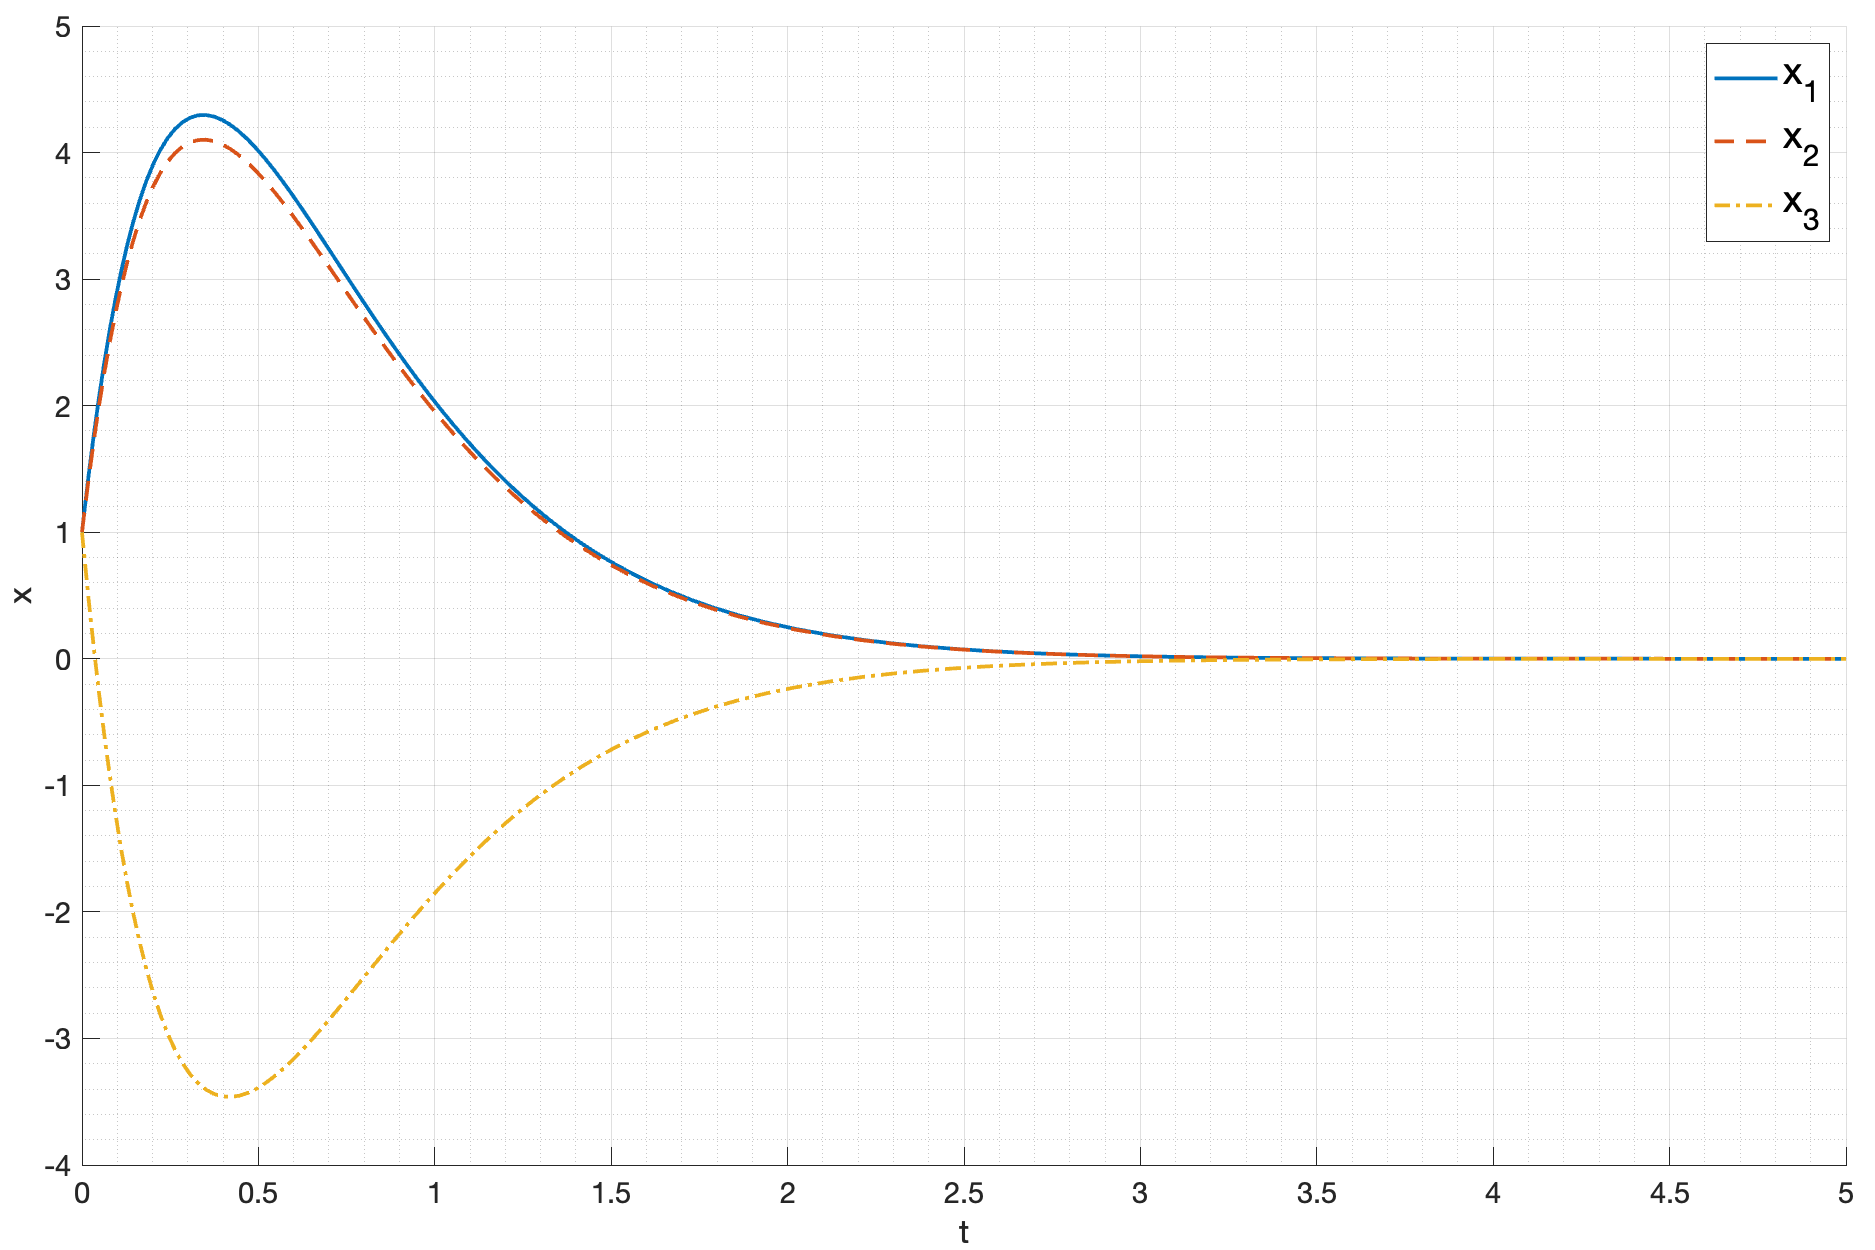
\includegraphics[width=\textwidth]{media/plots/task3_1_x.png}
    \caption{Состояние системы с регулятором $K_1$}
    \label{fig:task3_1_x}
\end{figure}
\begin{figure}[ht!]
    \centering
    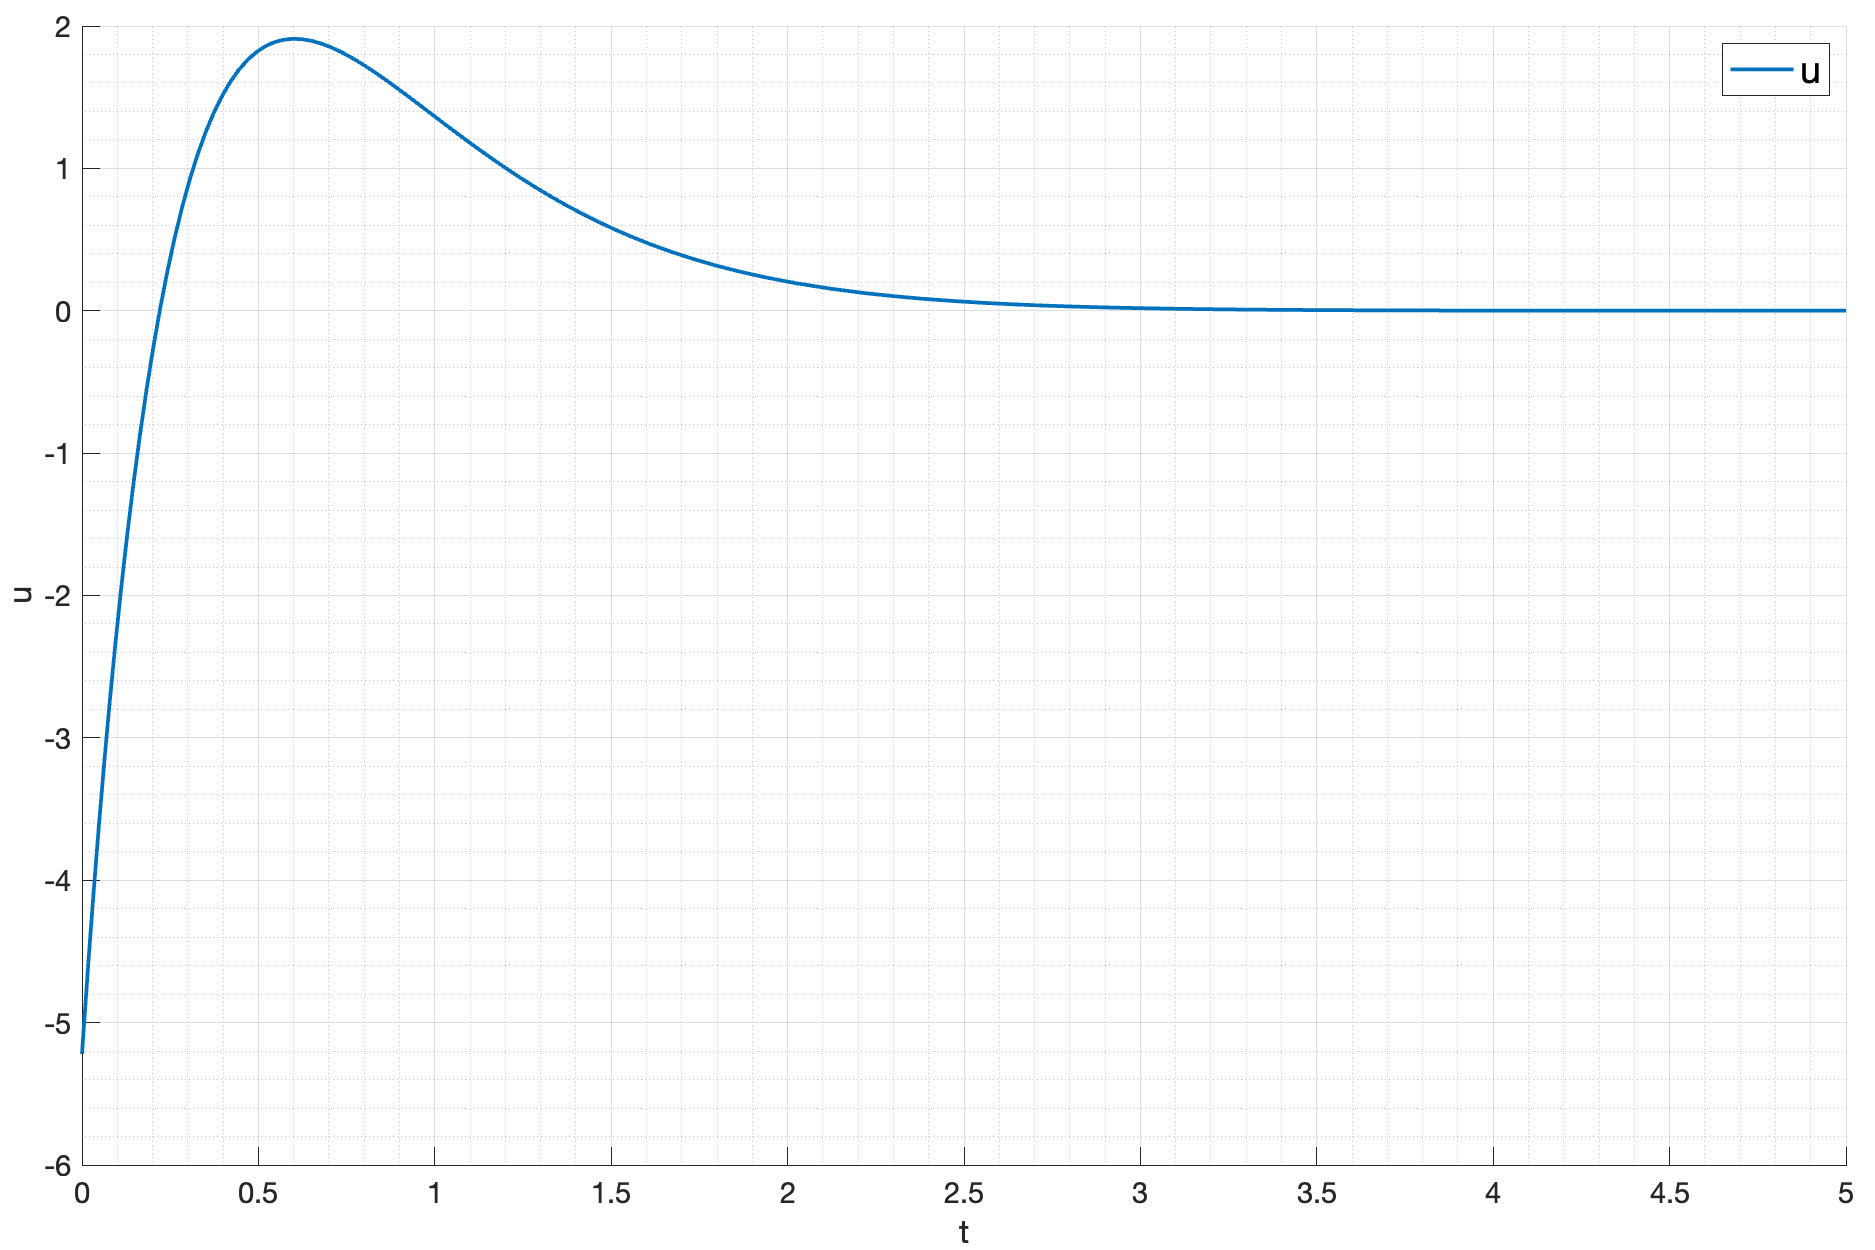
\includegraphics[width=\textwidth]{media/plots/task3_1_u.png}
    \caption{Управляющее воздействие системы с регулятором $K_1$}
    \label{fig:task3_1_u}
\end{figure}

Для системы с регулятором $K_2$ результаты моделирования представлены на рисунке \ref{fig:task3_2_x} 
(состояние системы) и \ref{fig:task3_2_u} (управляющее воздействие).

\begin{figure}[ht!]
    \centering
    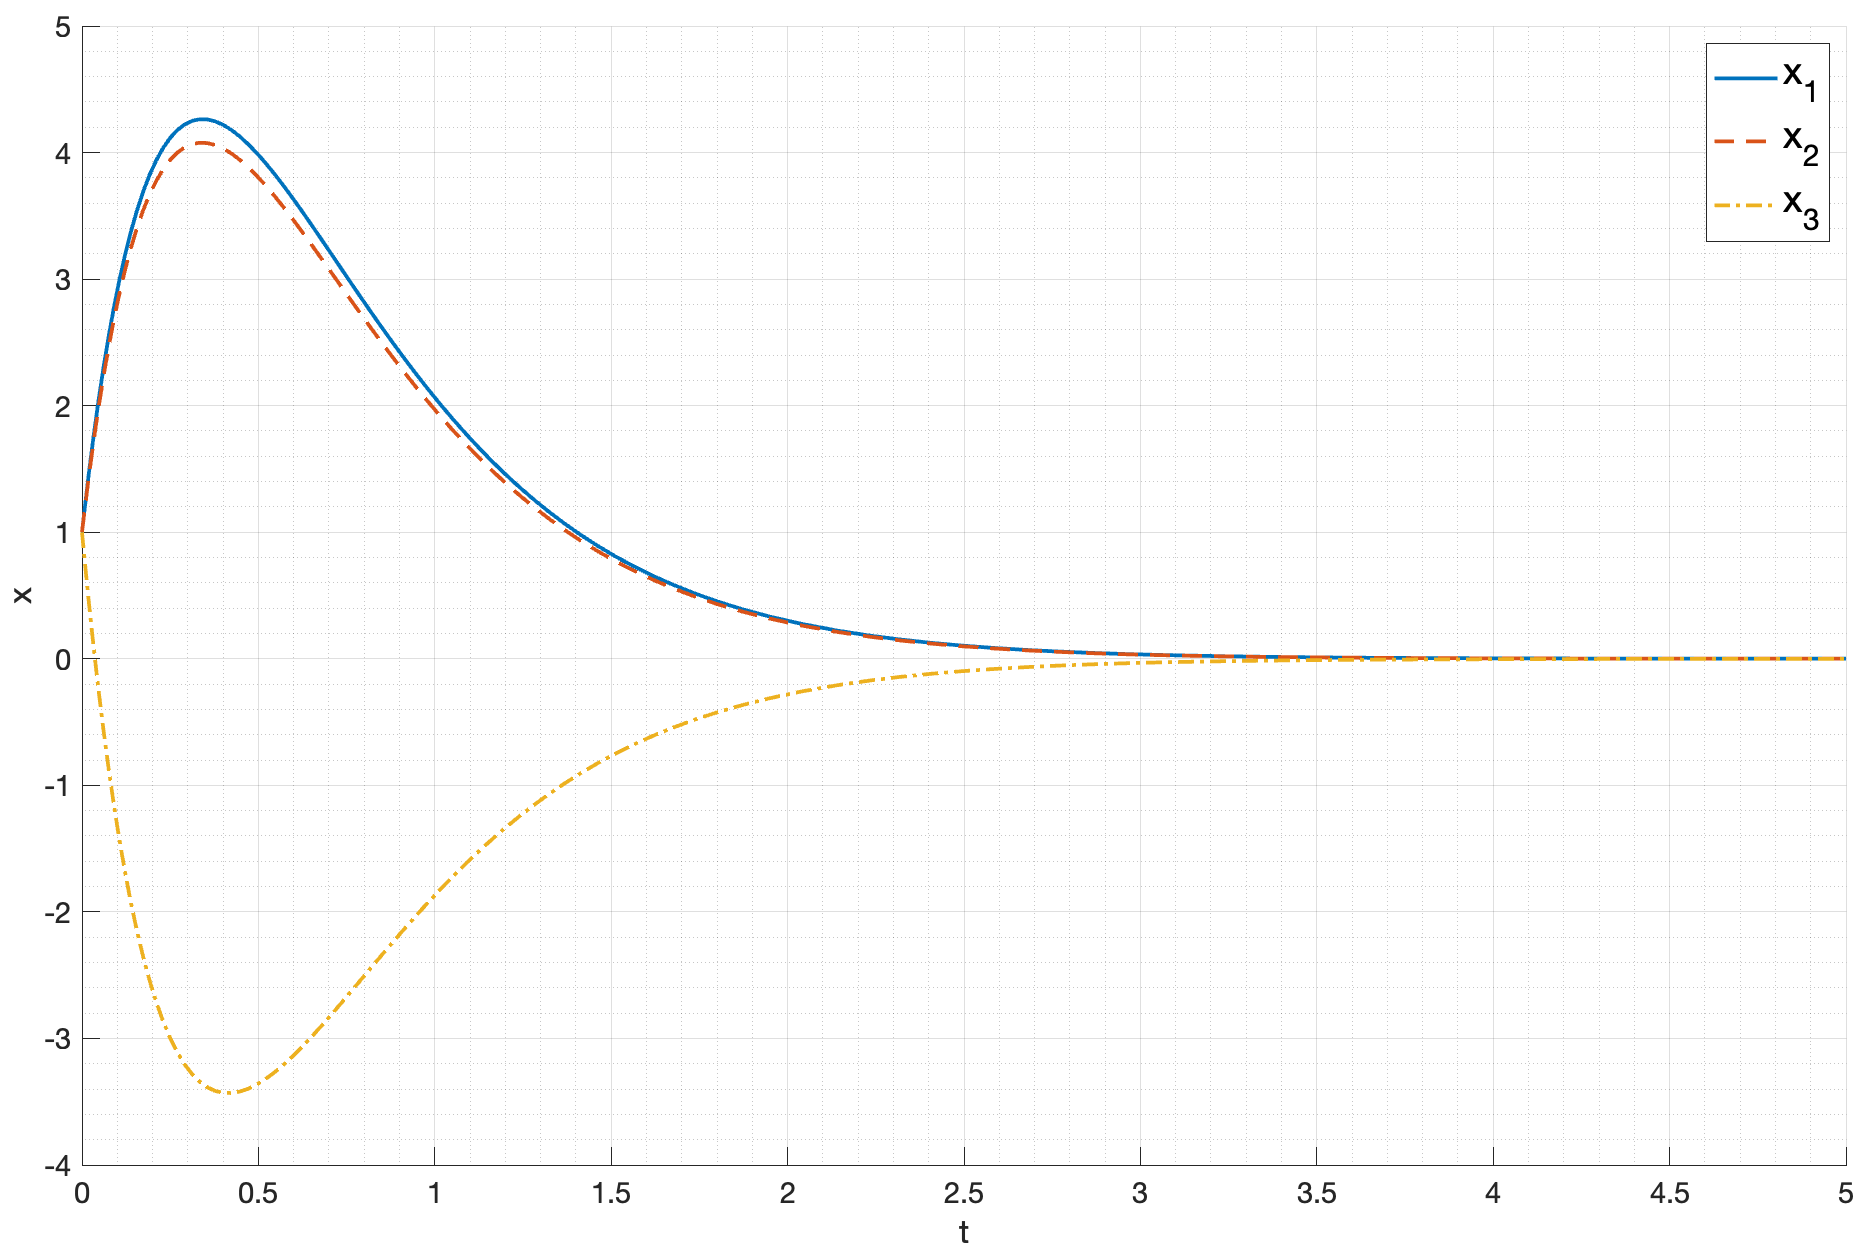
\includegraphics[width=\textwidth]{media/plots/task3_2_x.png}
    \caption{Состояние системы с регулятором $K_2$}
    \label{fig:task3_2_x}
\end{figure}
\begin{figure}[ht!]
    \centering
    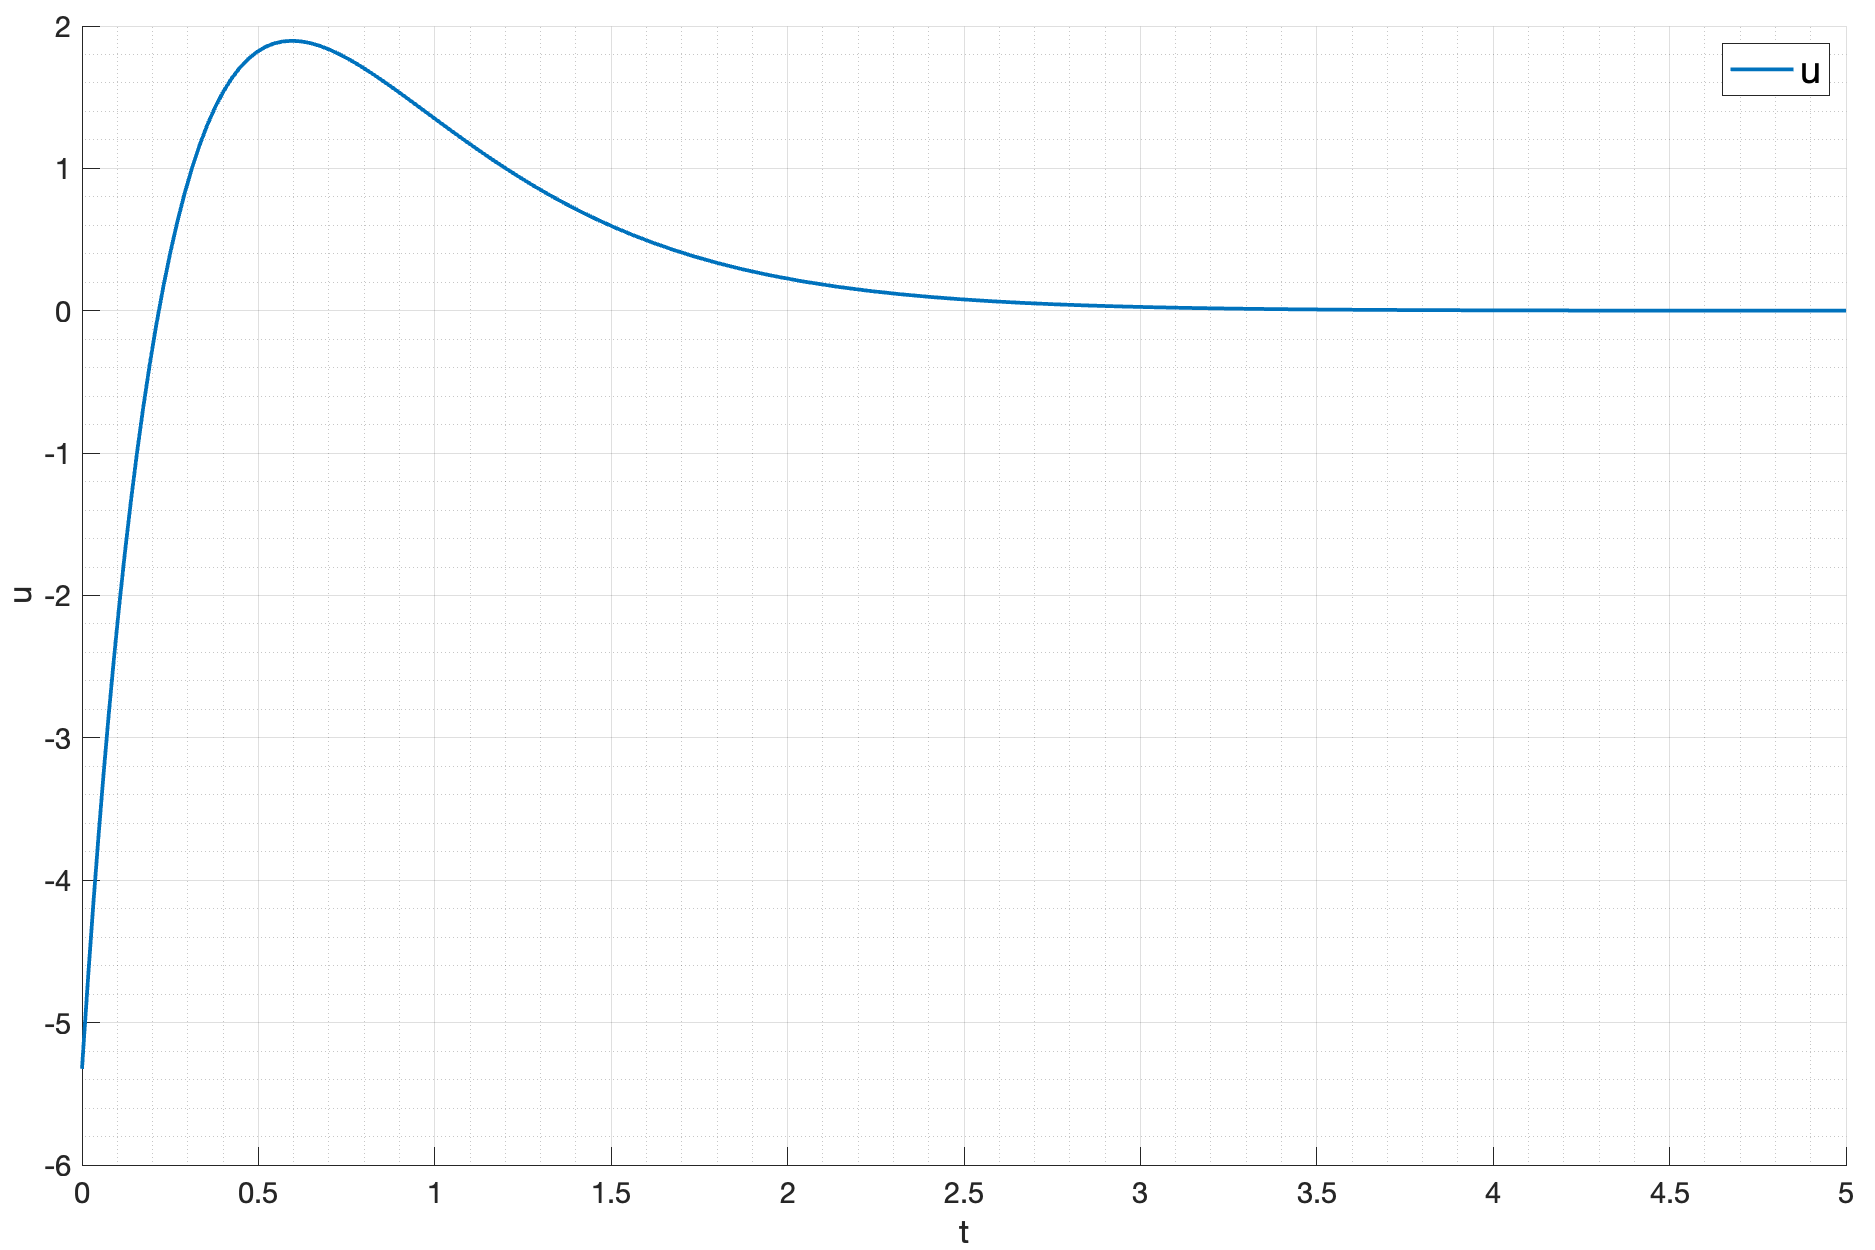
\includegraphics[width=\textwidth]{media/plots/task3_2_u.png}
    \caption{Управляющее воздействие системы с регулятором $K_2$}
    \label{fig:task3_2_u}
\end{figure}

Для системы с регулятором $K_3$ результаты моделирования представлены на рисунке \ref{fig:task3_3_x} 
(состояние системы) и \ref{fig:task3_2_u} (управляющее воздействие).

\begin{figure}[ht!]
    \centering
    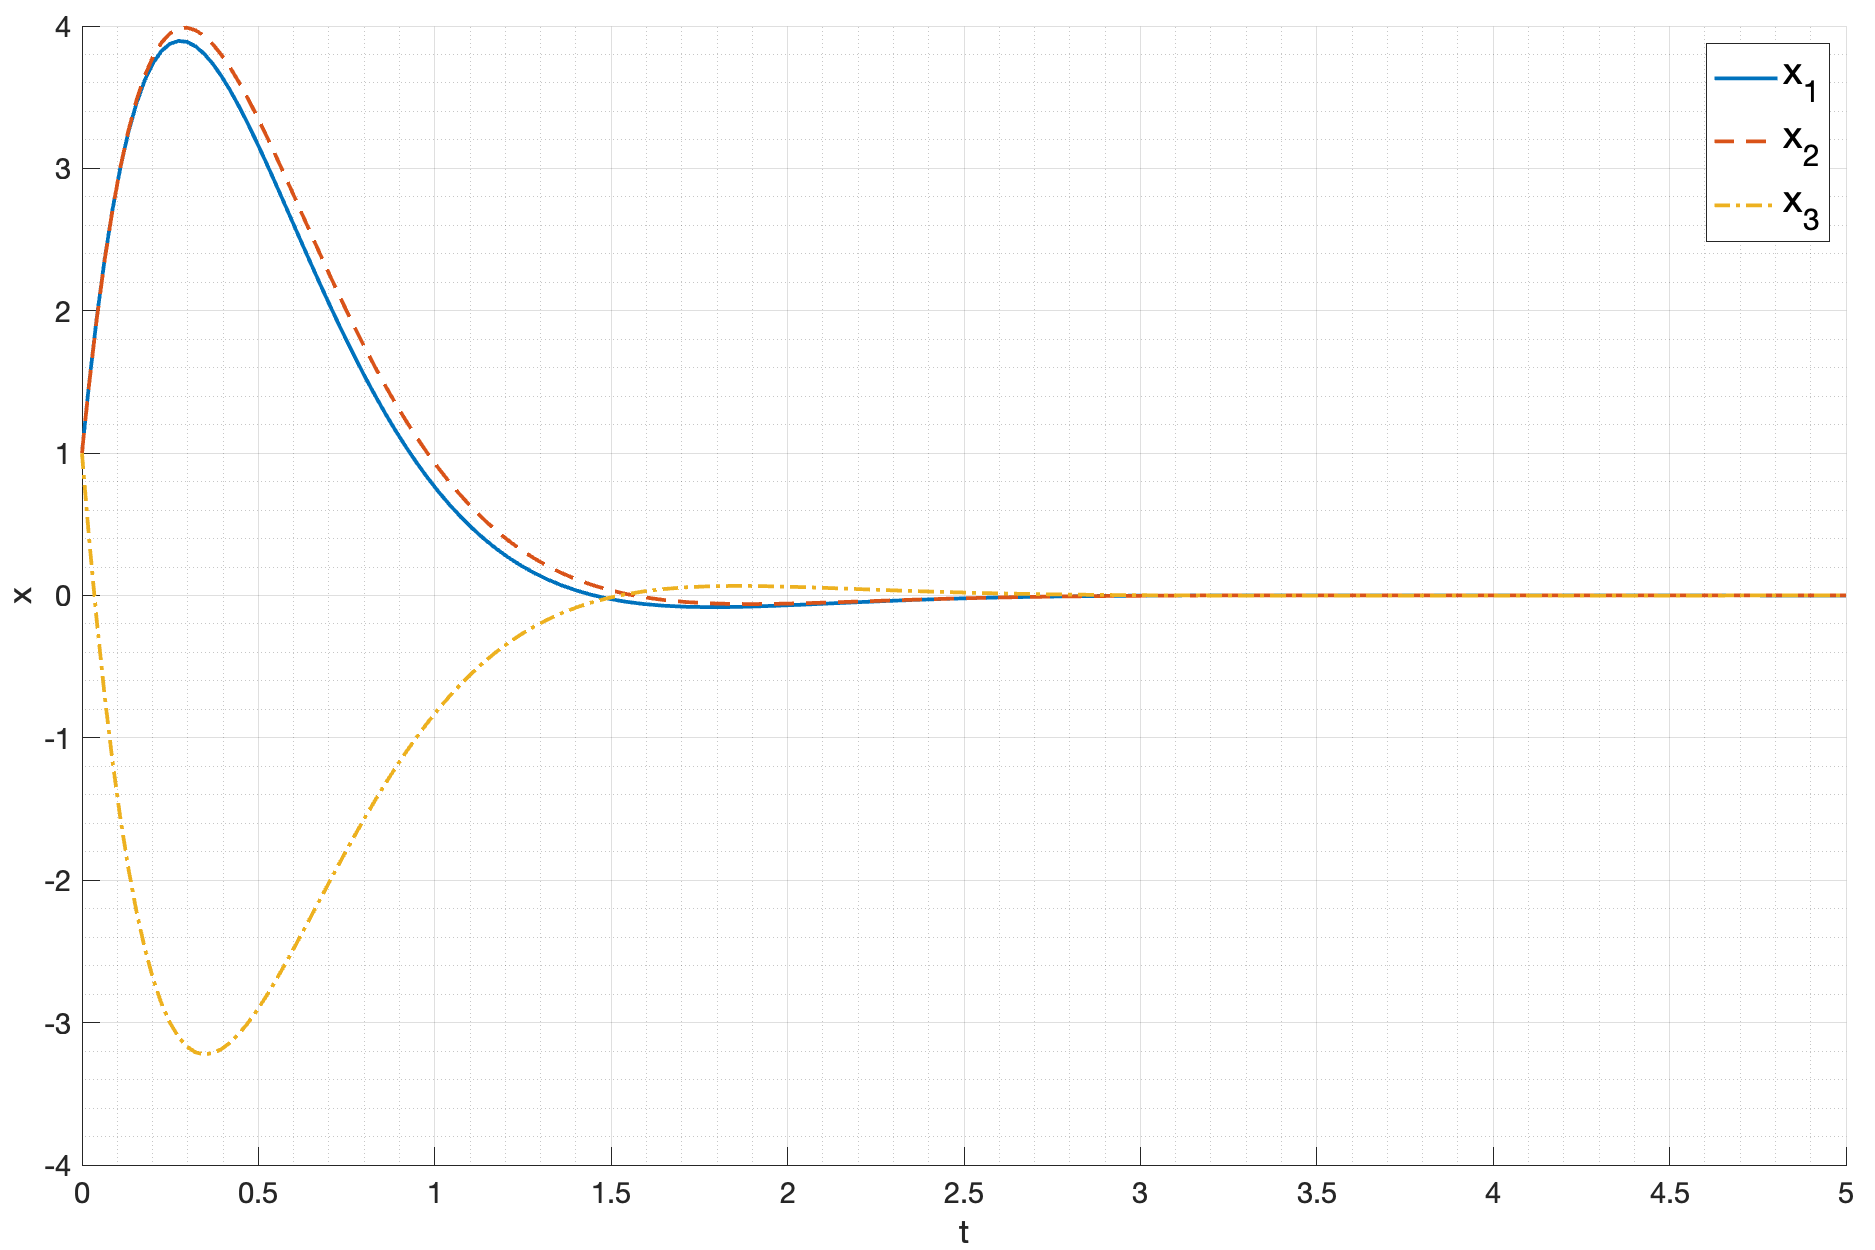
\includegraphics[width=\textwidth]{media/plots/task3_3_x.png}
    \caption{Состояние системы с регулятором $K_3$}
    \label{fig:task3_3_x}
\end{figure}
\begin{figure}[ht!]
    \centering
    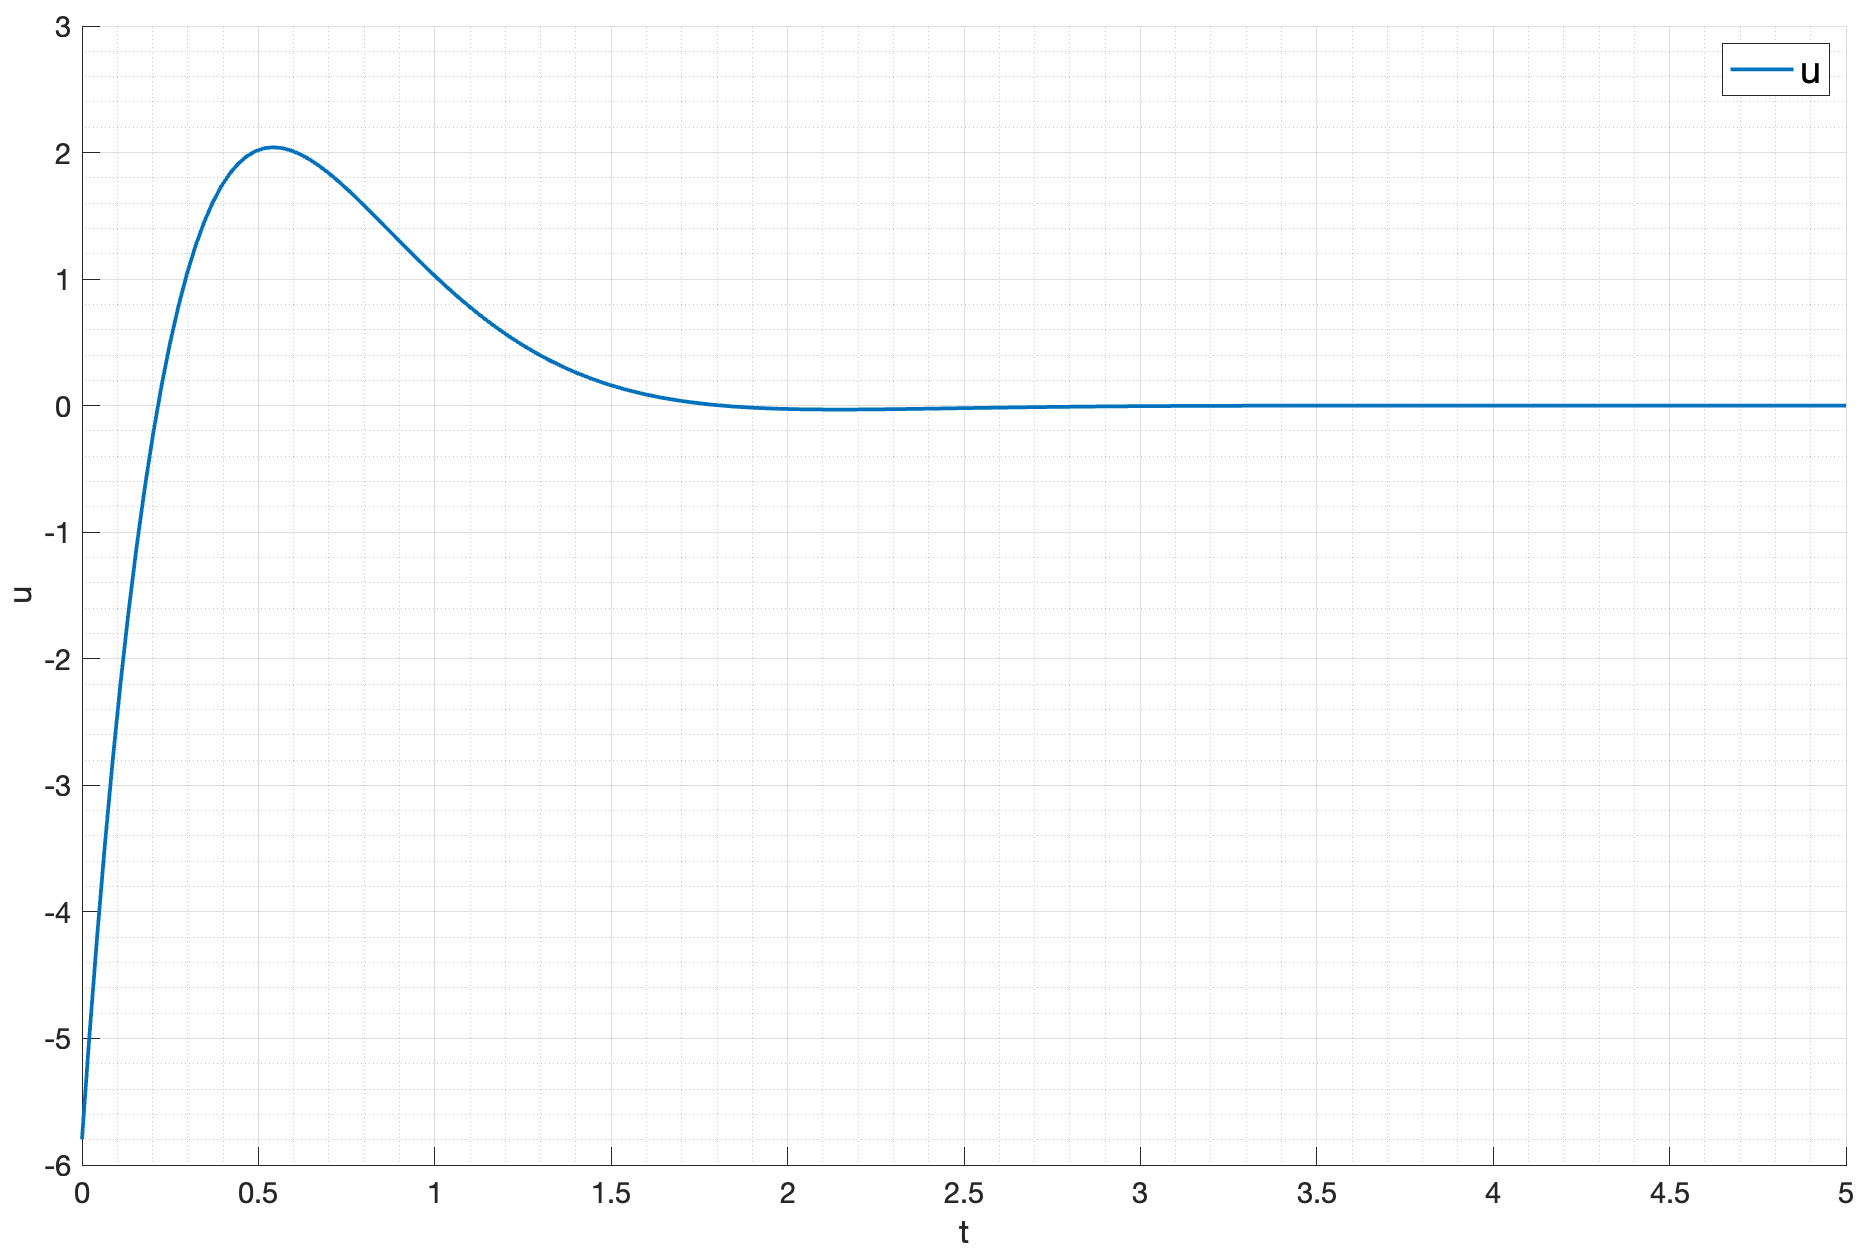
\includegraphics[width=\textwidth]{media/plots/task3_3_u.png}
    \caption{Управляющее воздействие системы с регулятором $K_3$}
    \label{fig:task3_3_u}
\end{figure}

Для системы с регулятором $K_4$ результаты моделирования представлены на рисунке \ref{fig:task3_4_x} 
(состояние системы) и \ref{fig:task3_4_u} (управляющее воздействие).
\begin{figure}[ht!]
    \centering
    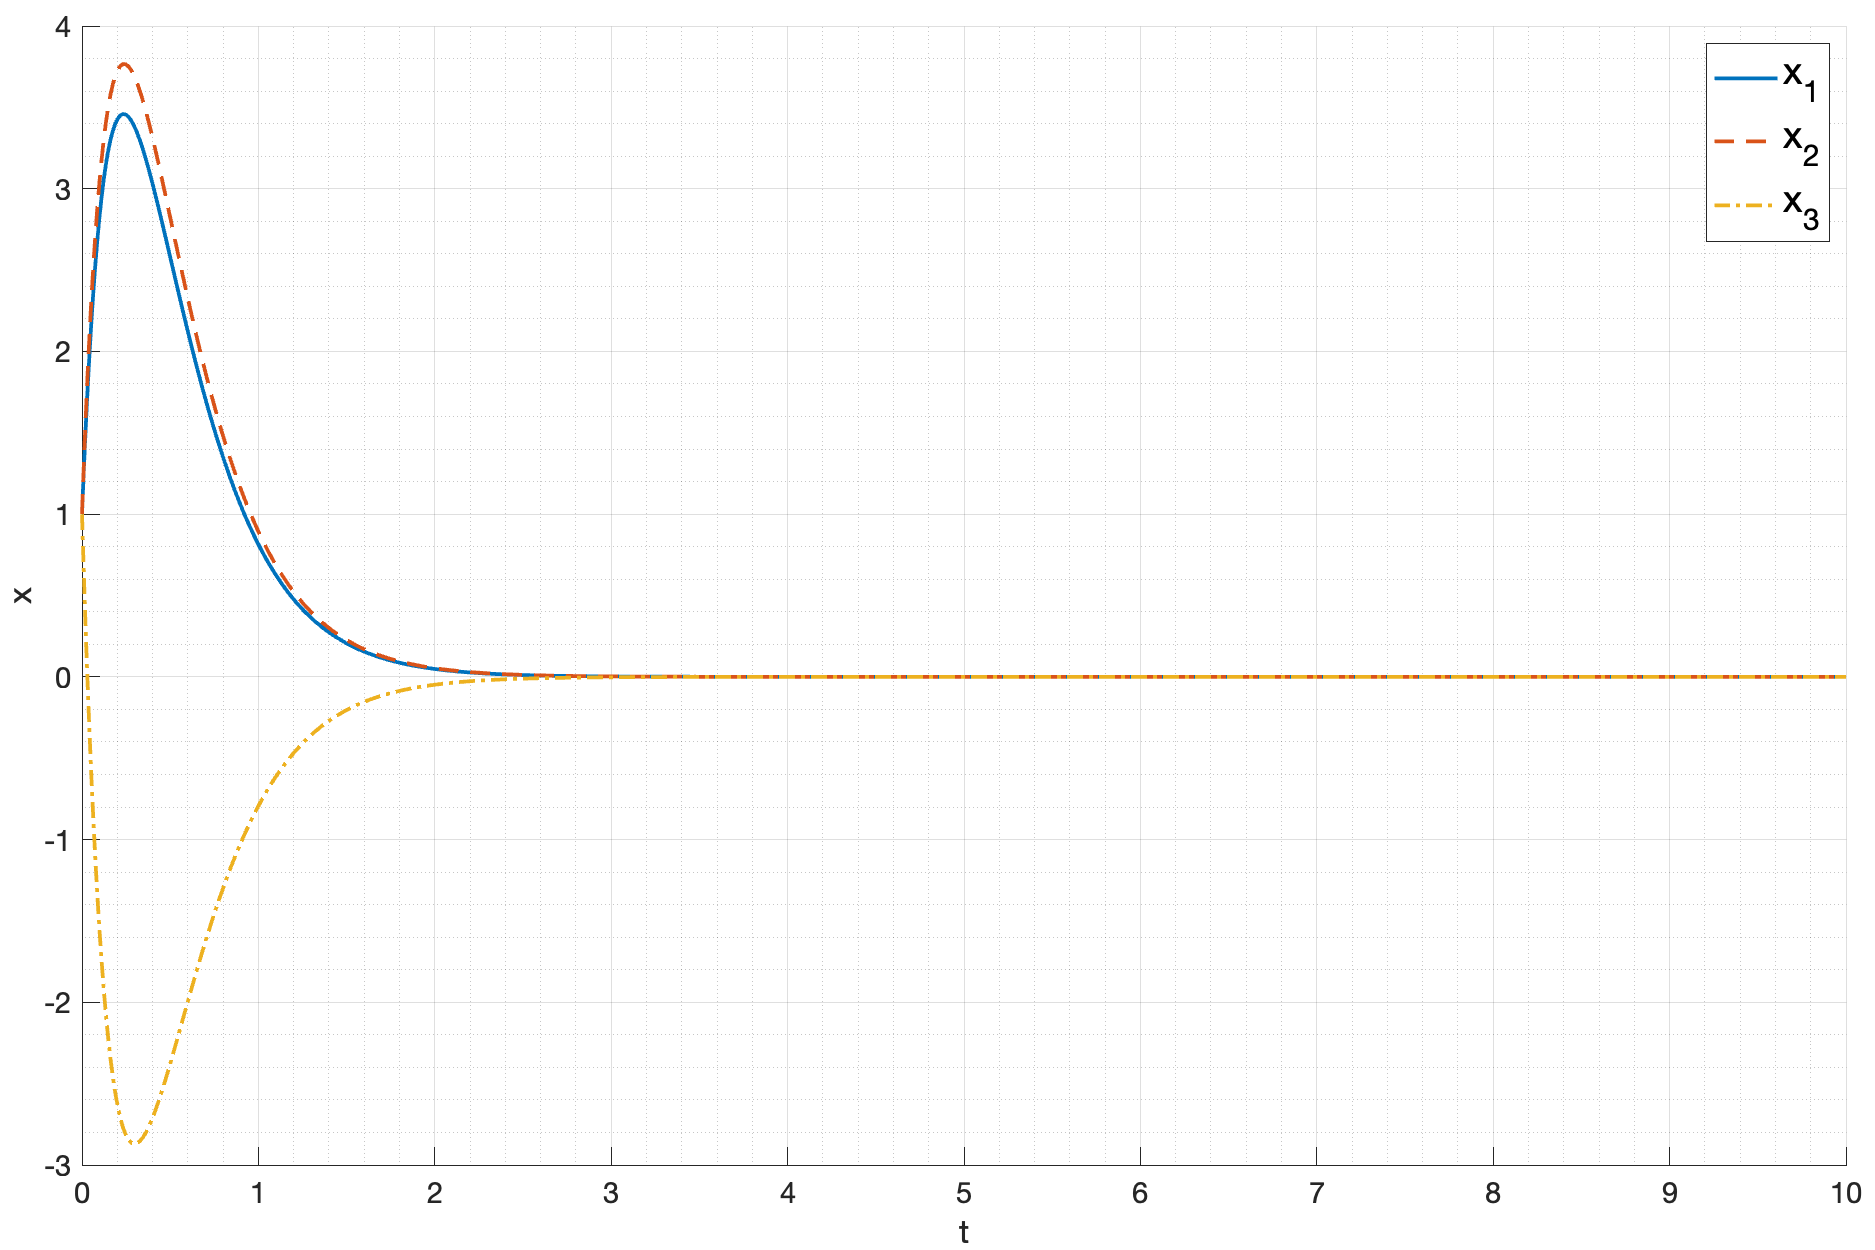
\includegraphics[width=\textwidth]{media/plots/task3_4_x.png}
    \caption{Состояние системы с регулятором $K_4$}
    \label{fig:task3_4_x}
\end{figure}

\begin{figure}[ht!]
    \centering
    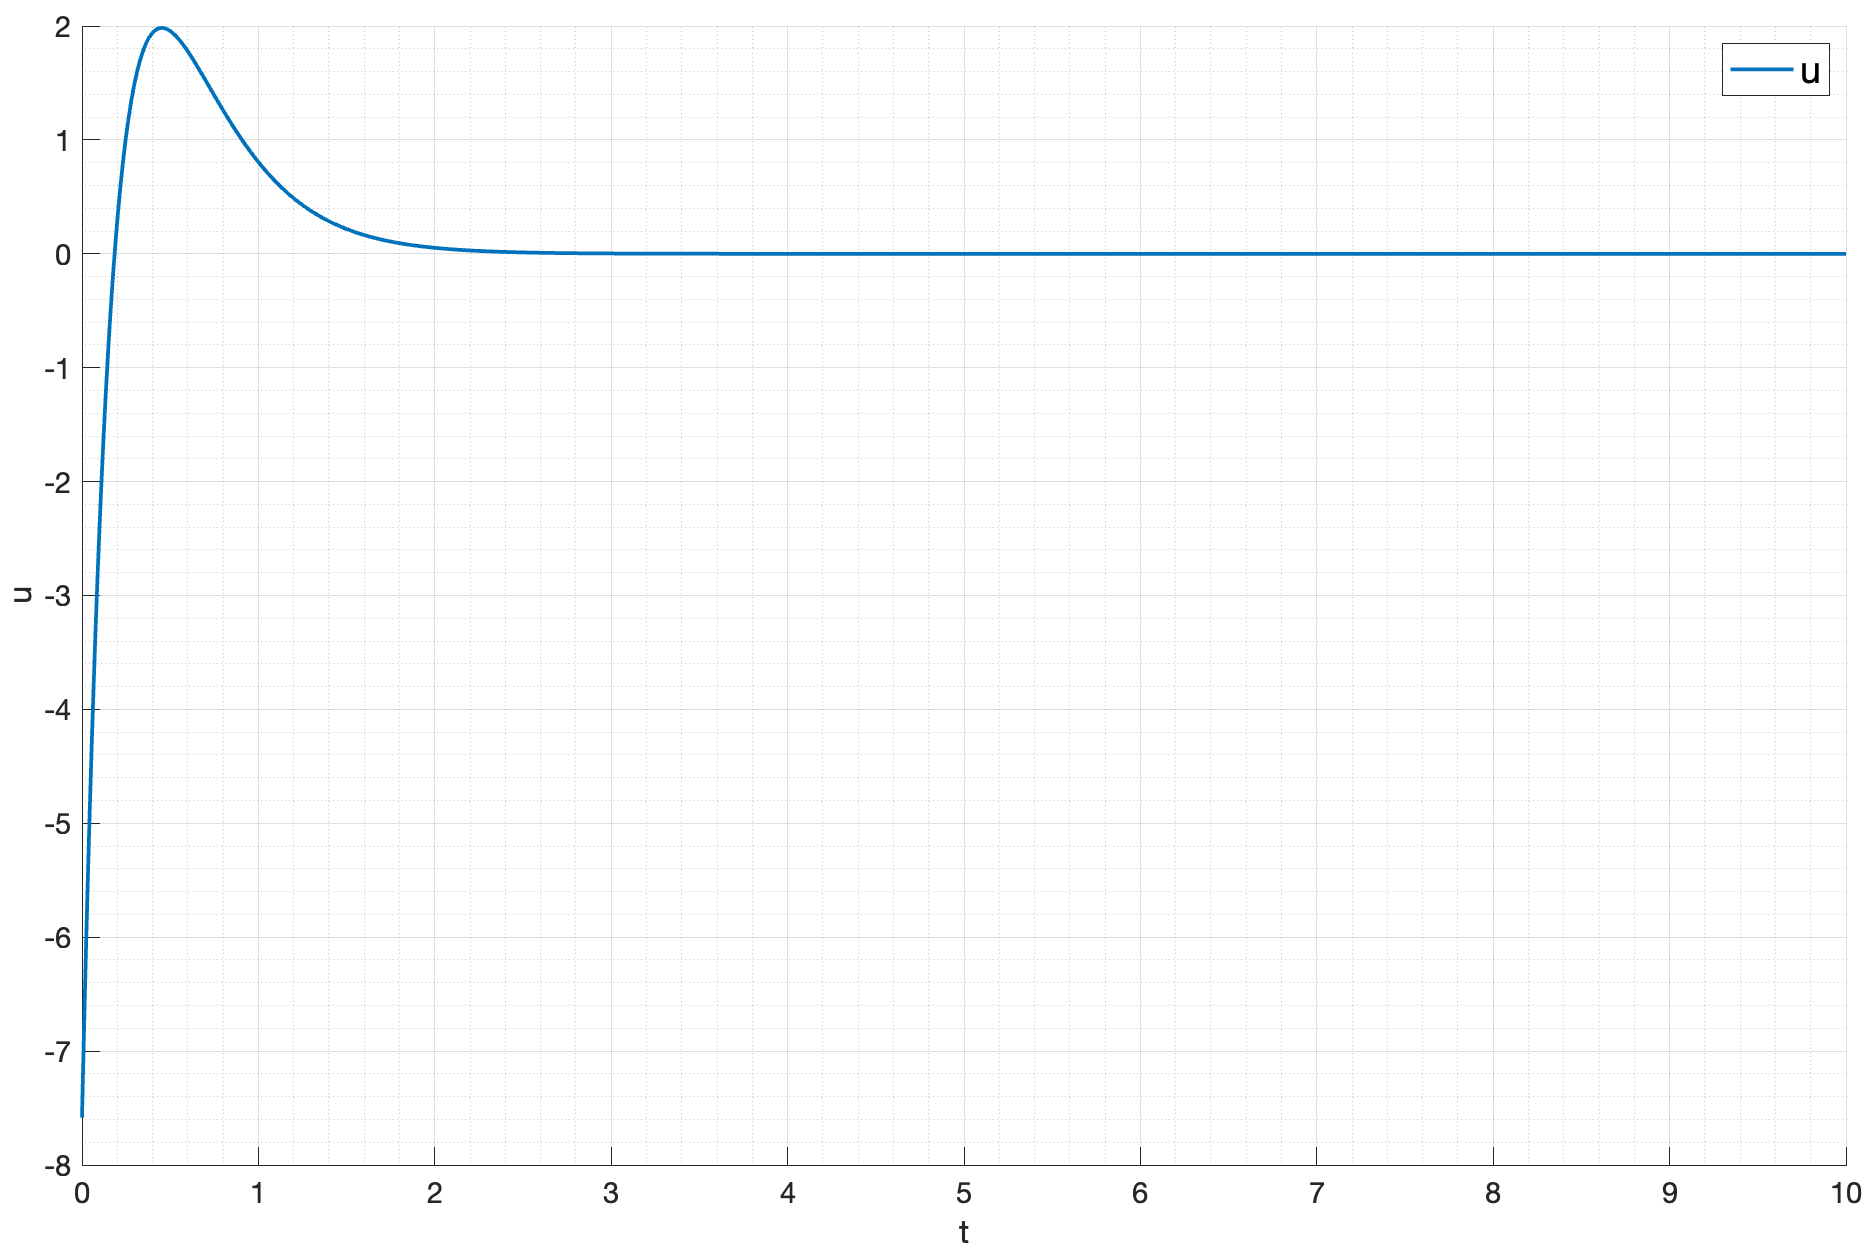
\includegraphics[width=\textwidth]{media/plots/task3_4_u.png}
    \caption{Управляющее воздействие системы с регулятором $K_4$}
    \label{fig:task3_4_u}
\end{figure}

\FloatBarrier
\subsection{Выводы}
В данном пункте был рассмотрен регулятор с качественной экспоненциальной устойчивостью, 
то есть регулятор, обеспечивающий заданное отклонение от средней траектории системы. Это наглядно 
демонстрируется на комплексной плоскости, где собственные числа системы располагаются внутри окружности,
центрированной в точке $\beta$ и радиусом $r$.
Матрица $Q$ определяет штраф на вектор состояния, а матрица $R$ -- штраф на управляющее воздействие.
При $Q = I$ система сходится быстрее к нулю, чем при $Q = 0$, 
При $R = 1$ управляющее воздействие не вызывает резких изменений в системе, аналогично 
оптимизации управления в предыдущих заданиях. 
\FloatBarrier

\section{Выводы}
В данной работы были рассмотрены различные методы анализа и моделирования динамических систем
без входного воздействия. Результаты показали, что динамику системы можно 
предсказать аналитически, использую корневой метод (корни характеристического уравнения). 
Так же, использую тот же метод, можно оценить область устойчивости системы. 
Последнее задание показало, что собственные числа матрицы управления системы в 
форме вход-состояние-выход совпадают с корнями характеристического уравнения. 
Используя этот факт можно осуществить управление системой, приведя ее к желаемому виду.